\documentclass[10pt,a4paper]{article}
\usepackage[utf8]{inputenc}
\usepackage[T1]{fontenc}
\usepackage[spanish, es-tabla]{babel}
\usepackage{lmodern}
\usepackage{csquotes}
\usepackage{amsmath, amsfonts, amssymb, amsthm}

\usepackage{graphicx}
\usepackage{subcaption}
\usepackage{float}

\usepackage[
    left=2.54cm,
    right=2.54cm,
    top=2.54cm,
    bottom=2.54cm
]{geometry}

\usepackage{xcolor}
\usepackage[most]{tcolorbox}
\usepackage{soul}

\usepackage{listings}
\usepackage{upquote}

\lstset{
    basicstyle=\footnotesize\ttfamily,
    frame=single,
    numbers=left,
    numberstyle=\tiny\color{gray},
    numbersep=8pt,
    inputencoding=utf8,
    extendedchars=true,
    breaklines=true,
    breakatwhitespace=false,
    showstringspaces=false,
    keepspaces=true,
    keywordstyle=\color{blue},
    commentstyle=\color{green!50!black},
    stringstyle=\color{red!70!black},
    tabsize=4
}
\usepackage{tikz}

\usetikzlibrary{
    arrows.meta,
    positioning,
    automata
}

\usepackage[
    colorlinks=true,
    linkcolor=blue!50!black,
    urlcolor=blue!60!black,
    citecolor=blue!50!black
]{hyperref}

%================================================
% CAJA DE EJERCICIOS
%================================================
\newtcbtheorem[number within=section]
{ejercicio}{Ejercicio}{
    enhanced,
    sharp corners,
    boxrule=0pt,
    leftrule=5pt,
    colframe=gray!30!black,
    colback=gray!5!white,
    coltitle=white,
    fonttitle=\bfseries,
    separator sign={.\ },
    before skip=10pt,
    after skip=10pt
}{ej}

%================================================
% CAJA DE TEOREMAS
%================================================
\newtcbtheorem[number within=section]
{mytheo}{Teorema}{
    enhanced,
    sharp corners,
    boxrule=0pt,
    leftrule=5pt,
    colframe=blue!40!black,
    colback=blue!5!white,
    coltitle=white,
    fonttitle=\bfseries,
    separator sign={.\ },
    before skip=10pt,
    after skip=10pt
}{th}

%================================================
% CAJA DE ALERTA
%================================================
\newtcolorbox{alerta}[1]{
    enhanced,
    sharp corners,
    boxrule=0pt,
    leftrule=5pt,
    colframe=red!40!black,
    colback=red!5!white,
    coltitle=white,
    fonttitle=\bfseries,
    title={#1},
    before skip=10pt,
    after skip=10pt
}

%================================================
% CAJA DE NOTAS
%================================================
\newtcolorbox{nota}[1]{
    enhanced,
    sharp corners,
    boxrule=0pt,
    leftrule=5pt,
    colframe=orange!40!black,
    colback=yellow!5!white,
    coltitle=white,
    fonttitle=\bfseries,
    title={#1},
    before skip=10pt,
    after skip=10pt
}


\begin{document}

\begin{titlepage}
    \centering

    %========================================
    % UNIVERSIDAD
    %========================================
    {\huge\textbf{Universidad Nacional Autónoma de México}}

    \vspace{0.3cm}
    \rule{\linewidth}{2mm}

    \vspace{0.3cm}
    {\large\textbf{Facultad de Estudios Superiores Acatlán}}

    \vspace{0.8cm}

    %========================================
    % LOGOTIPOS
    %========================================
    \noindent
    \begin{minipage}{0.45\textwidth}
        \centering
        \IfFileExists{../../../../Archivos/Imagenes_Logos/acatlan.png}{
            
\includegraphics[
                width=5cm,
                height=4cm,
                keepaspectratio
            ]{../../../../Archivos/Imagenes_Logos/acatlan.png}
        }{
            \textit{Logotipo FES Acatlán}
        }
    \end{minipage}
    \hfill
    \begin{minipage}{0.45\textwidth}
        \centering
        \IfFileExists{../../../Archivos/Imagen/LOGO_DBA.png}{
            
\includegraphics[
                width=5cm,
                height=4cm,
                keepaspectratio
            ]{../../../Archivos/Imagen/LOGO_DBA.png}
        }{
            \textit{Logotipo DBA}
        }
    \end{minipage}

    \vspace{0.8cm}

    %========================================
    % CARRERA Y TÍTULO
    %========================================
 

    \vspace{0.8cm}
    {\huge\textbf{Database Administrator}}

    \vspace{0.4cm}
    \rule{\linewidth}{1mm}

    \vspace{0.4cm}

    %========================================
    % PROYECTOS
    %========================================
    {\Large\textbf{Empresa - Proyecto}}

    \vspace{0.3cm}
    {\large\textit{Query Teach Solutions}}

    \vspace{0.2cm}
    {\large\textit{Movilidad: Ecobici CDMX}}

    \vspace{6cm}

    %========================================
    % INTEGRANTES
    %========================================
    \rule{\linewidth}{0.5mm}

    \vspace{0.3cm}
    {\large\textbf{Integrantes}}

    \vspace{0.3cm}
    {\large Estrada Romero Meliza Edith}

    \vspace{0.15cm}
    {\large Ricardo López Ramírez}

    \vspace{0.15cm}
    {\large Ruiz Sánchez Emiliano}

    \vspace{0.15cm}
    {\large Cabrera Trejo José Luis}

    \vspace{0.5cm}
    \rule{\linewidth}{0.5mm}

    \vspace{0.5cm}

    %========================================
    % FECHA
    %========================================
    {\small Actualización: \today}

\end{titlepage}


%================================================
% ÍNDICE
%================================================
\pagenumbering{roman}

\tableofcontents

\clearpage

%================================================
% CONTENIDO
%================================================
\pagenumbering{arabic}
\setcounter{page}{1}

\section{Tema y Descripción del Proyecto}

\subsection{Descripción General}
\textbf{Movilidad Urbana: Análisis del Sistema Ecobici en la Ciudad de México}, 
consiste en el diseño, estructuración e implementación de una base de datos relacional 
analítica enfocada en la red de transporte de bicicletas de la CDMX. Un diseño de arquitectura basada en 
un Modelo de Estrella, el proyecto procesa y normaliza un volumen masivo de datos transaccionales 
correspondientes a los años 2024, 2025 y 2026. 

\subsection{Elección del Tema}
Se seleccionó este tema porque el sistema Ecobici es fundamental de la movilidad sustentable y el desarrollo
urbano en la capital del país. 
La Data proporcionada por Ecobici CDMX, genera un volumen de información masivo diariamente. 
Esto nos presentó un escenario ideal, para aplicar técnicas avanzadas de administración de bases de datos. 
Resolver las limitantes de particionamiento del motor de bases de datos mientras se garantizaba un 
100\% de integridad referencial, demuestra el nivel técnico requerido para gestionar 
arquitecturas de datos.

\subsection{Información a Visualizar en la Base de Datos}
La base de datos está estructurada para visualizar la interacción entre los usuarios y el sistema de movilidad mediante las siguientes dimensiones y métricas:
\begin{itemize}
    \item \textbf{Hechos de Movilidad:} Más de 6.5 millones de registros operativos en la tabla principal y más de 30 millones en el histórico, detallando cada viaje realizado.
    \item \textbf{Perfiles Demográficos:} Género y edad de los usuarios, permitiendo segmentar el comportamiento del consumidor.
    \item \textbf{Dimensión Espacial:} Catálogo de estaciones de retiro y arribo, incluyendo su nomenclatura y zonificación, para trazar las rutas urbanas.
    \item \textbf{Dimensión Temporal:} Fechas exactas y franjas horarias (Mañana, Tarde, Noche, Madrugada) para identificar horas pico y valles de demanda.
    \item \textbf{Inventario Físico:} Estatus y tipo de las bicicletas utilizadas.
\end{itemize}


\begin{table}[h]
\centering
\caption{Volumetría de Datos del Proyecto}
\vspace{0.2cm}
\begin{tabular}{|l|c|l|}
\hline
\textbf{Tabla / Entidad} & \textbf{Tipo en Modelo} & \textbf{Volumen Aproximado} \\ \hline
Historico Viajes & Tabla Particionada & $> 30,000,000$ registros \\ \hline
Viajes (2025-2026) & Tabla de Hechos & $> 6,500,000$ registros \\ \hline
Estaciones & Catálogo / Dimensión & 683 estaciones únicas \\ \hline
Tiempos & Dimensión Temporal & 86,400 segundos \\ \hline
\end{tabular}
\label{tab:volumetria}
\end{table}

\subsection{Finalidad Principal}
La finalidad principal de esta base de datos no es únicamente el almacenamiento, es servir  
como un repositorio analítico. 
El objetivo es transformar los datos en información estratégica que permita a la toma de decisiones 
optimizar la logística del sistema.
Mediante las sentencias DML, la base de datos es capaz de responder 
preguntas de negocio en segundos.
Ejemplo: la saturación de las estaciones por franjas horarias, 
los patrones de ruta más frecuentes según el género del usuario.

\newpage

\section{Diagrama Entidad-Relación}

\begin{figure}[h]
    \centering
    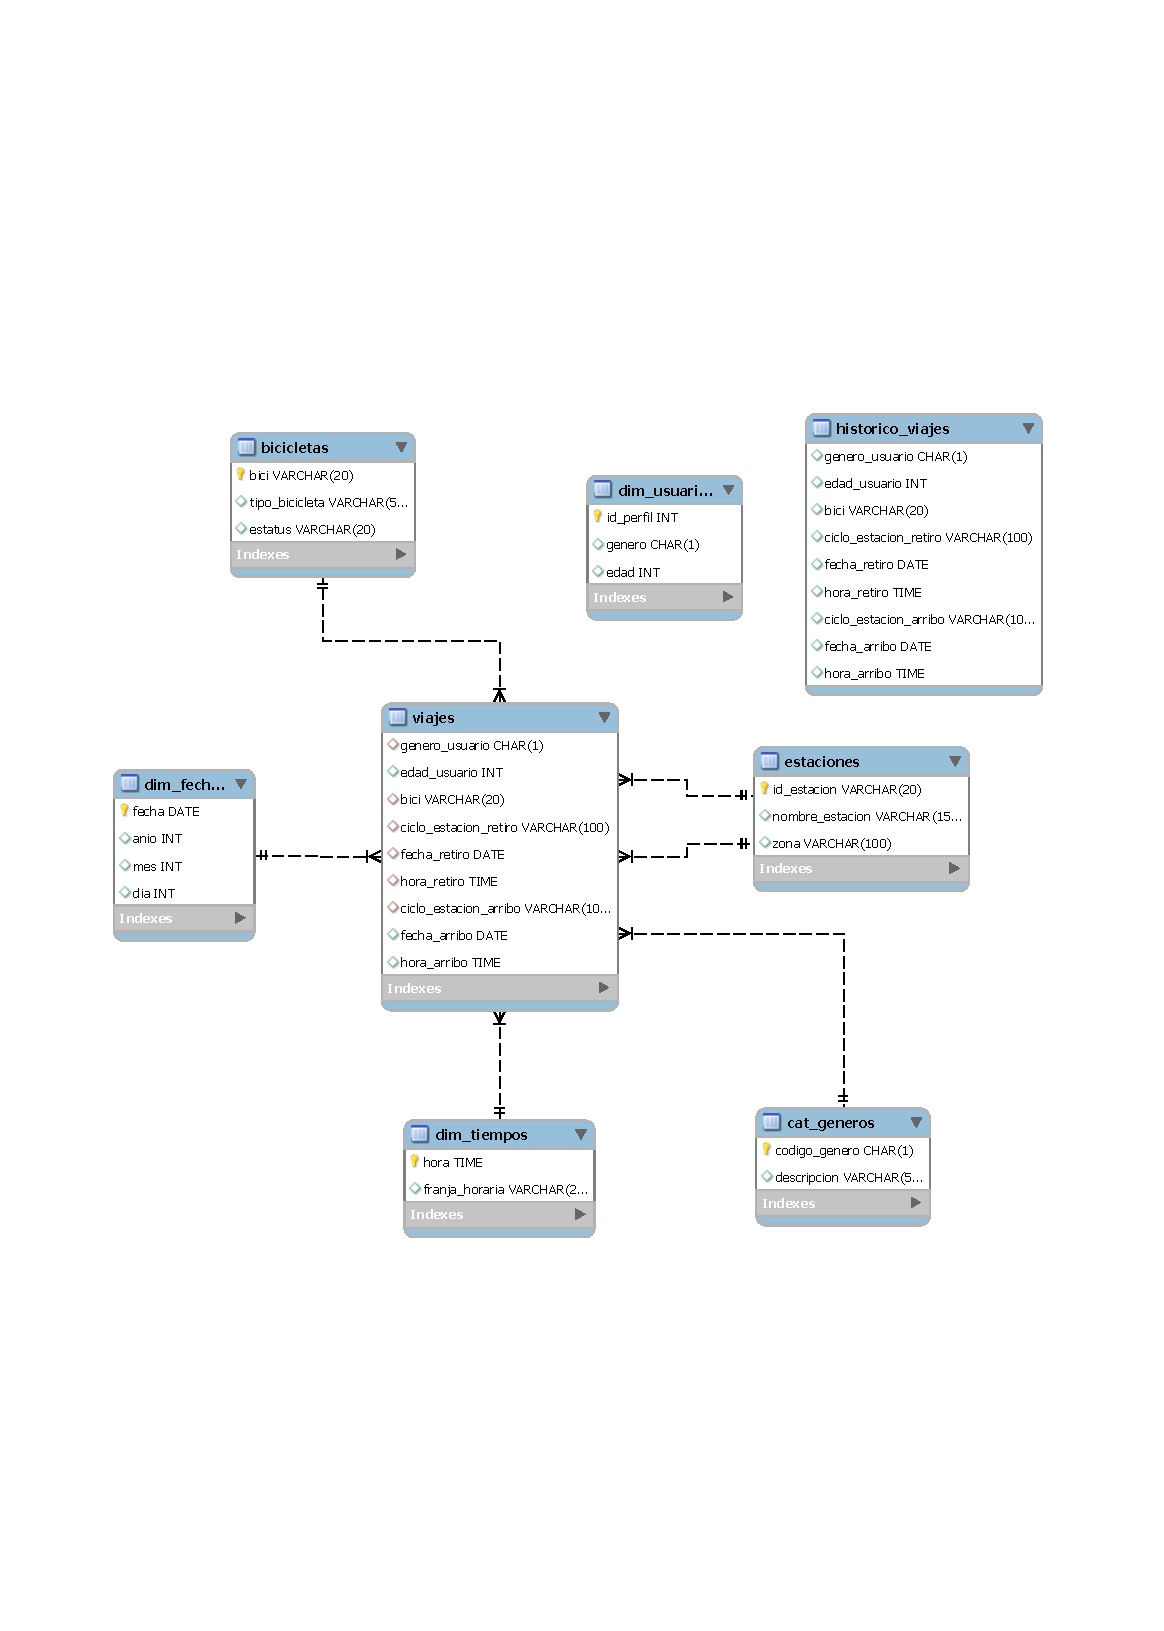
\includegraphics[width=0.8\textwidth]{../Diagrama_EER_Ecobici.pdf}
    \caption{Diagrama Entidad-Relación (Modelo de Estrella) estructurado para el análisis.}
    \label{fig:diagrama_eer}
\end{figure}


\newpage

\section{Enlace a Repositorio GitHub.}

\vspace{5mm}

\begin{center}
    \href{https://github.com/Richard-0x/db-administration}{
        \fbox{\rule{0pt}{12pt}\hspace{8pt}\textbf{Repositorio GitHub}\hspace{8pt}}
    }
\end{center}

\section{Enlace Google Drive}

\vspace{5mm}

\begin{center}
    \href{https://drive.google.com/drive/folders/1ogxHLMOxqbDtDr0JjjXlNfBxNryxPC8Q?usp=sharing}{
        \fbox{\rule{0pt}{12pt}\hspace{8pt}\textbf{DATA DRIVE}\hspace{8pt}}
    }
\end{center}



\newpage 
\section{Estimación Teórica y Proyección de Espacio en Disco LocalHost.}
\subsection{1. Tamaño por tipo de dato y fila (Row Size)}
Para realizar la estimación de espacio, se sumaron los bytes requeridos por cada columna de las tablas principales (\texttt{viajes}, \texttt{historico\_viajes}, \texttt{dim\_usuarios}, \texttt{estaciones}, etc.), utilizando los pesos estándar de MySQL: \texttt{INT} = 4 bytes, \texttt{DATETIME} = 5 bytes, \texttt{SMALLINT} = 2 bytes y \texttt{TINYINT} = 1 byte.

A esto se sumó la sobrecarga (\textit{overhead}) interna de InnoDB: encabezado de fila ($\sim$5 bytes), ID de transacción (6 bytes) y puntero de rollback (7 bytes). Considerando el tamaño por defecto de la página InnoDB (16 KB) y un \textit{fill factor} de 15/16, se determinó que la fila promedio ocupa aproximadamente \textbf{70 bytes} (incluyendo índices B-Tree de las Claves Primarias y Foráneas).

\subsection{2. Cálculo del Espacio de Carga Inicial}
Con la fila promedio de 70 bytes, se proyectó la carga inicial antes de la inyección física de datos:
\begin{itemize}
    \item \textbf{Carga Inicial de \texttt{historico\_viajes}} ($\sim$30,000,000 registros): $\sim$2.1 GB de datos + $\sim$1.2 GB de índices = \textbf{$\sim$3.3 GB}.
    \item \textbf{Carga Inicial de \texttt{viajes}} ($\sim$6,500,000 registros): $\sim$455 MB de datos + $\sim$260 MB de índices = \textbf{$\sim$715 MB}.
    \item \textbf{Catálogos y Dimensiones:} \textbf{$\sim$15 MB}.
    \item \textbf{Total Carga Inicial:} \textbf{$\sim$4.03 GB}.
\end{itemize}

\subsection{3. Simulación y Proyección de Crecimiento}
Asumiendo un promedio de 800,000 viajes mensuales nuevos en la CDMX y un incremento anual estimado del 10\% debido a nuevas estaciones. El crecimiento mensual proyectado es: 800,000 $\times$ 100 bytes (datos + índices) $\approx$ 80 MB/mes (lo que equivale a $\sim$0.96 GB/año).

\begin{table}[H]
\centering
\begin{tabular}{|l|c|}
\hline
\textbf{Periodo} & \textbf{Almacenamiento Estimado} \\ \hline
Año 1 (Actual / Carga Inicial) & 4.03 GB \\ \hline
Año 2 (+10\% uso) & $\sim$5.08 GB \\ \hline
Año 3 (+20\% uso) & $\sim$6.24 GB \\ \hline
Año 5 (+40\% uso) & $\sim$8.95 GB \\ \hline
\end{tabular}
\caption{Tabla de Proyección a 5 Años}
\end{table}


\newpage 
\section{Consulta Diccionario de Datos y Comparación de Almacenamiento LocalHost.}
\subsection{Justificación Teórica}
En MySQL 8.0, los metadatos se almacenan de forma centralizada y transaccional en el Diccionario de Datos. Medir los archivos físicos (como \texttt{.ibd}) directamente desde el sistema operativo resulta impreciso debido a dos factores:
\begin{itemize}
    \item \textbf{Asignación por Extents:} El motor InnoDB reserva espacio en bloques completos, por lo que el archivo en disco siempre será más grande que los datos reales almacenados.
    \item \textbf{Fragmentación:} El espacio de los registros eliminados no se devuelve inmediatamente al sistema operativo.
\end{itemize}
Por ello, consultar el \texttt{INFORMATION\_SCHEMA} permite al administrador medir el espacio lógico real, exacto y en uso.

\subsection{Desarrollo de Consultas SQL}

\textbf{A. Tamaño total de la Base de Datos}
\begin{lstlisting}
    SELECT table_schema AS Base_de_Datos,
    ROUND(SUM(data_length + index_length) / 1024 / 1024, 2) AS Tamano_MB
    FROM information_schema.tables
    WHERE table_schema = 'DB_Ecobici_CDMX'
    GROUP BY table_schema;
\end{lstlisting}

\begin{figure}[H]
    \centering
    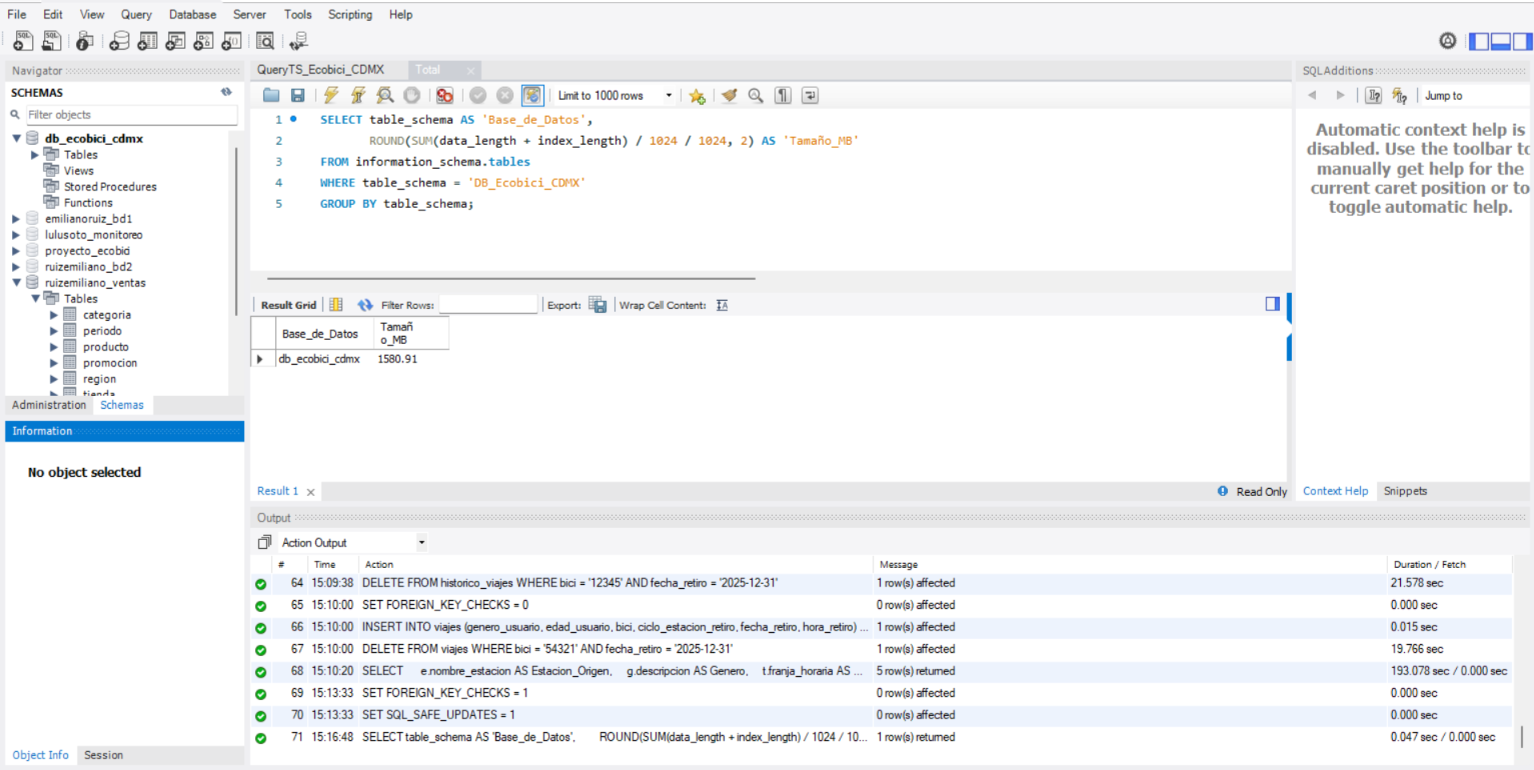
\includegraphics[width=0.8\textwidth]{../../../Archivos/Imagen/img_total.png}
    \caption{Tamaño total de la base de datos.}
\end{figure}

Como se observa en el resultado, el tamaño lógico total del esquema \texttt{DB\_Ecobici\_CDMX} es de \textbf{1580.91 MB} (aproximadamente 1.58 GB). Este valor representa la suma exacta de los datos puros más el peso de los índices, confirmando que la carga masiva de los registros se completó exitosamente.

\vspace{0.5cm}
\textbf{B. Tamaño individual por tabla e índice}
\begin{lstlisting}[language=SQL]
SELECT table_name AS `Tabla`,
       ROUND(data_length / 1024 / 1024, 2) AS `Datos_MB`,
       ROUND(index_length / 1024 / 1024, 2) AS `Indices_MB`,
       table_rows AS `Numero_Registros`
FROM information_schema.tables
WHERE table_schema = 'DB_Ecobici_CDMX'
ORDER BY (data_length + index_length) DESC;
\end{lstlisting}

\begin{figure}[H]
    \centering
    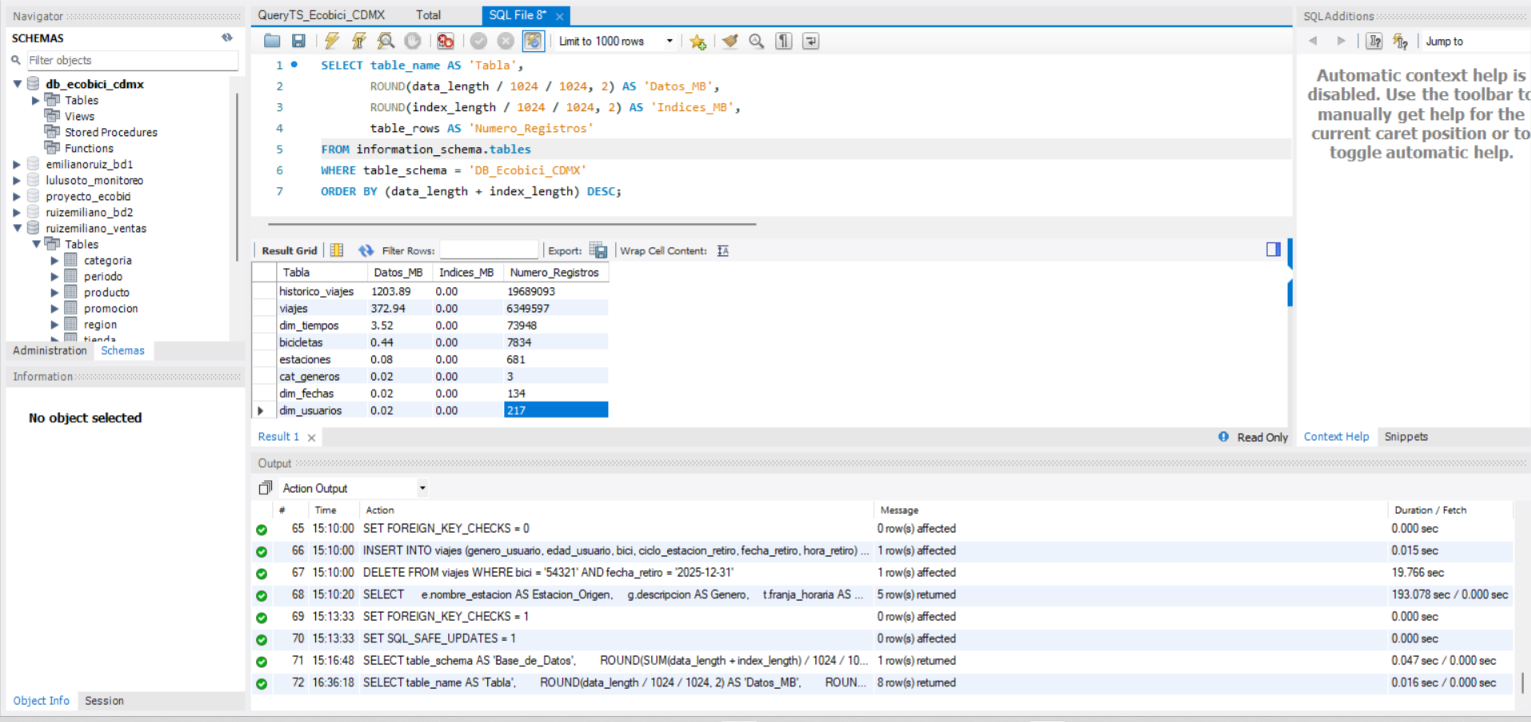
\includegraphics[width=0.8\textwidth]{../../../Archivos/Imagen/img_tablas.png}
    \caption{Desglose de peso por datos e índices de cada tabla.}
\end{figure}

\vspace{0.5cm}
\textbf{C. Consulta de Tablespaces y archivos .ibd}
\begin{lstlisting}[language=SQL]
SELECT TABLESPACE_NAME AS `Particion_Tablespace`,
       FILE_NAME AS `Ruta_Archivo_ibd`,
       ROUND(TOTAL_EXTENTS * EXTENT_SIZE / 1024 / 1024, 2) AS `Espacio_Asignado_MB`,
       ROUND(FREE_EXTENTS * EXTENT_SIZE / 1024 / 1024, 2) AS `Espacio_Libre_MB`
FROM information_schema.FILES
WHERE TABLESPACE_NAME LIKE 'DB_Ecobici_CDMX/historico_viajes%';
\end{lstlisting}

\begin{figure}[H]
    \centering
    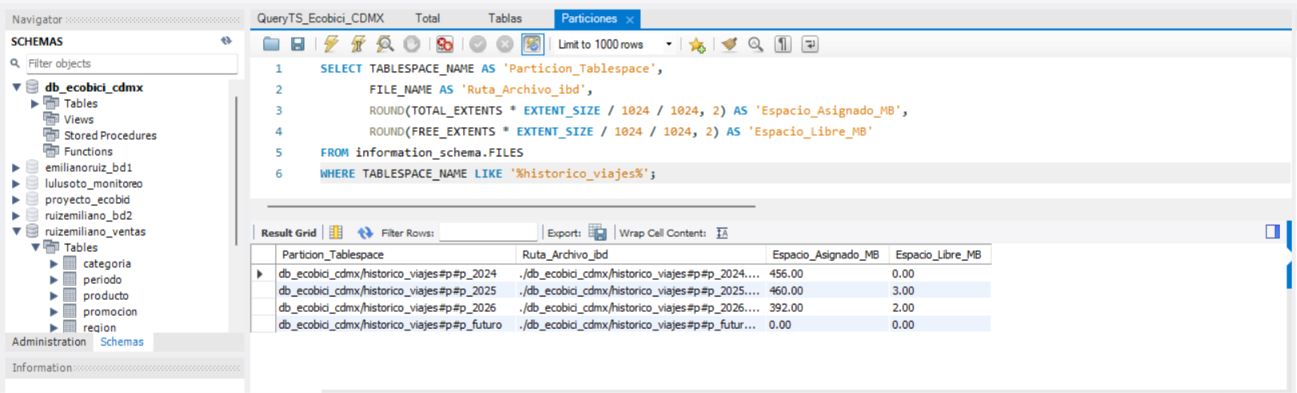
\includegraphics[width=0.8\textwidth]{../../../Archivos/Imagen/img_particiones.png}
    \caption{Espacio físico asignado vs libre en las particiones de la tabla histórica.}
\end{figure}

\subsection{Matriz de Comparación}
El siguiente cuadro contrasta la estimación matemática contra la medición real del Diccionario de Datos.

\begin{table}[H]
\centering
\begin{tabular}{|l|c|c|c|c|}
\hline
\textbf{Tabla} & \textbf{Filas (Aprox)} & \textbf{Teórico (MB)} & \textbf{Real (MB)} & \textbf{Diferencia} \\ \hline
historico\_viajes & 19,689,093 & 3379.20 & 1203.89 & -2175.31 \\ \hline
viajes & 6,349,597 & 715.00 & 372.94 & -342.06 \\ \hline
Catálogos (Suma) & 82,683 & 15.00 & 4.10 & -10.90 \\ \hline
\end{tabular}
\caption{Comparativa Estimación Teórica vs Diccionario de Datos}
\end{table}

\textbf{Análisis:} El tamaño real resultó menor a la estimación teórica principalmente porque el modelo matemático calculó la tabla histórica sobre 30 millones de registros, mientras que la carga física procesó aproximadamente 20 millones.


\newpage



\section{Aseguramiento de la Disponibilidad y Automatización LocalHost}

La replicación configurada en la Sección 1.3 protege al sistema contra la caída de un servidor, pero no contra errores lógicos. Por ejemplo, si un usuario ejecuta por error un \texttt{DELETE} sobre la tabla de viajes, la réplica aplica ese mismo borrado en cuestión de segundos. Por esta razón, la replicación no sustituye a los respaldos.

Para garantizar la continuidad y el mantenimiento del motor, se diseñó una estrategia operativa automatizada con cuatro ejes: respaldos programados, mantenimiento preventivo, purga y rotación de datos, y monitoreo. Las tareas se programan durante la madrugada, cuando la operación de Ecobici es mínima, y se ordenan para evitar que varios procesos pesados coincidan.

\subsection{Calendario operativo}

\begin{table}[htbp]
    \centering
    \small
    \begin{tabular}{|p{4.2cm}|p{3.2cm}|p{3.6cm}|p{2cm}|}
        \hline
        \textbf{Tarea} & \textbf{Herramienta} & \textbf{Frecuencia} & \textbf{Hora (CDMX)} \\ \hline
        Respaldo incremental (binlogs) & \texttt{cron} + \texttt{docker cp} & Diario & 00:50 \\ \hline
        Respaldo completo & \texttt{cron} + \texttt{mysqldump} & Semanal (domingo) & 03:00 \\ \hline
        Rotación de particiones & \texttt{cron} & Mensual (primer sábado) & 01:00 \\ \hline
        \texttt{ANALYZE TABLE} & Event Scheduler & Semanal (sábado) & 03:00 \\ \hline
        \texttt{OPTIMIZE TABLE viajes} & Event Scheduler & Mensual (primer sábado) & 03:00 \\ \hline
        Purga de binlogs & MySQL (automática) & Continua, 14 días & --- \\ \hline
        Reporte de monitoreo & \texttt{cron} & Diario & 07:00 \\ \hline
    \end{tabular}
    \caption{Calendario de tareas automatizadas.}
    \label{tab:calendario-operativo}
\end{table}

El primer sábado de cada mes, la rotación de particiones se ejecuta a la 01:00 y el mantenimiento a las 03:00. Este orden permite que el mantenimiento se ejecute después de la rotación. El respaldo completo del domingo se programa en un día distinto al mantenimiento del sábado.

\newpage

\subsection{Estrategia de respaldos}

La estrategia combina dos tipos de respaldo: un respaldo lógico \textbf{completo} cada semana y una copia diaria de los registros binarios (\textit{binary logs} o \textit{binlogs}). El respaldo completo representa una fotografía de la base de datos; los binlogs registran los cambios posteriores. En conjunto, y siempre que la cadena de archivos esté completa y sea consistente, permiten recuperar la información hasta un punto determinado en el tiempo (\textit{Point-in-Time Recovery}, PITR).

\paragraph{Respaldo completo semanal.}
El respaldo se ejecuta con \texttt{mysqldump} desde la réplica para reducir la carga de lectura sobre el servidor principal. Las opciones exactas deben validarse con la versión de MySQL utilizada y con la configuración GTID del entorno. El ejemplo siguiente presupone que las credenciales se gestionan de forma segura y que los directorios de destino ya existen.

\begin{lstlisting}
#!/bin/bash
# Respaldo logico completo semanal (domingo 03:00)
set -o pipefail

FECHA=$(date +%Y-%m-%d)
DIR="$HOME/proyecto_ecobici"
ARCHIVO="$DIR/backups/completos/ecobici_completo_${FECHA}.sql.gz"

if docker exec mysql-slave mysqldump \
    --defaults-extra-file=/run/secrets/mysql-client.cnf \
    --single-transaction --source-data=2 --set-gtid-purged=ON \
    --routines --triggers --events \
    --databases DB_Ecobici_CDMX | gzip > "$ARCHIVO"; then
    echo "$(date) OK respaldo completo: $ARCHIVO" >> "$DIR/logs/respaldos.log"
else
    echo "$(date) ERROR en respaldo completo" >> "$DIR/logs/respaldos.log"
    rm -f "$ARCHIVO"
    exit 1
fi

# Conservar aproximadamente las ultimas cuatro semanas
find "$DIR/backups/completos" \
    -name "ecobici_completo_*.sql.gz" -mtime +28 -delete
\end{lstlisting}

\textbf{Nota de seguridad:} el archivo de credenciales del ejemplo es ilustrativo. Debe existir dentro del contenedor, tener permisos restrictivos y configurarse según la imagen utilizada. No se recomienda guardar contraseñas directamente en el código ni publicarlas en el repositorio.

\newpage

\paragraph{Respaldo diario de binlogs.}
Cada noche se puede ejecutar \texttt{FLUSH BINARY LOGS} para cerrar el binlog actual y comenzar uno nuevo. Los archivos cerrados se copian fuera del contenedor; el archivo activo no debe copiarse mientras MySQL siga escribiéndolo. El ejemplo requiere que el usuario de MySQL tenga los permisos necesarios y que el directorio de destino exista.

\begin{lstlisting}
#!/bin/bash
# Copia diaria de binlogs (00:50)
set -euo pipefail

DIR="$HOME/proyecto_ecobici"
DESTINO="$DIR/backups/binlogs"
mkdir -p "$DESTINO"

# Se recomienda usar un archivo de opciones protegido.
MYSQL=(docker exec mysql-master mysql
       --defaults-extra-file=/run/secrets/mysql-client.cnf
       -N -e)

# 1. Rotar el binlog activo
"${MYSQL[@]}" "FLUSH BINARY LOGS;"

# 2. Identificar el archivo binlog activo
ACTIVO=$("${MYSQL[@]}" "SHOW BINARY LOG STATUS;" | awk 'NR==1 {print $1}')

# 3. Copiar binlogs cerrados que aun no existan en el destino
for f in $(docker exec mysql-master \
    sh -c "ls /var/lib/mysql | grep -E '^mysql-bin\\.[0-9]+$'"); do
    if [ "$f" != "$ACTIVO" ] && [ ! -f "$DESTINO/$f" ]; then
        docker cp "mysql-master:/var/lib/mysql/$f" "$DESTINO/"
        echo "$(date) Binlog copiado: $f" >> "$DIR/logs/respaldos.log"
    fi
done

# 4. Aplicar la retencion definida para las copias locales
find "$DESTINO" -type f -name "mysql-bin.*" -mtime +14 -delete
\end{lstlisting}

\textbf{Importante:} el nombre de la consulta de estado depende de la versión de MySQL. En versiones que no admitan \texttt{SHOW BINARY LOG STATUS}, debe utilizarse la sentencia equivalente disponible en esa versión. Además, la rotación y copia de binlogs debe coordinarse con la política de purga del servidor y con el estado de la réplica.

\newpage

\paragraph{Procedimiento de recuperación a un punto en el tiempo (PITR).}
Supóngase que el miércoles 21 de octubre de 2026 a las 15:00, hora de Ciudad de México, se ejecuta por error un \texttt{DELETE} que elimina los viajes de octubre. La recuperación debe realizarse en una instancia aislada, sin modificar directamente el servidor principal.

\begin{lstlisting}[language=bash, caption={Esquema de recuperación a un punto en el tiempo}]
# 1. Preparar una instancia aislada con la misma version compatible
# de MySQL y una configuracion de recuperacion validada.
docker run -d --name mysql-recuperacion \
    -e MYSQL_ROOT_PASSWORD='CAMBIAR_POR_UN_SECRETO_SEGURO' \
    mysql:8.0

# 2. Restaurar el respaldo completo correspondiente.
# El procedimiento exacto depende de las opciones GTID incluidas
# en el dump y del estado inicial de la instancia de recuperacion.
gunzip -c backups/completos/ecobici_completo_2026-10-18.sql.gz \
    | docker exec -i mysql-recuperacion \
      mysql -uroot -p

# 3. Copiar los binlogs disponibles al contenedor de recuperacion.
docker cp backups/binlogs/. mysql-recuperacion:/tmp/binlogs/

# 4. Inspeccionar y reproducir los binlogs en orden cronologico,
# deteniendose justo antes del momento del error.
# Verificar primero la zona horaria y el formato temporal de los logs.
# Ejemplo ilustrativo: ajustar los nombres de archivo y la hora real.
docker exec mysql-recuperacion sh -c \
  "mysqlbinlog --stop-datetime='2026-10-21 20:59:59' \
  /tmp/binlogs/mysql-bin.000001 /tmp/binlogs/mysql-bin.000002 \
  | mysql -uroot -p"
\end{lstlisting}

El comando anterior es un esquema de procedimiento, no una receta universal que deba ejecutarse sin validación. Antes de reproducir los binlogs, se debe confirmar su orden, la continuidad de la secuencia, la zona horaria y la compatibilidad de los GTID incluidos en el respaldo. La restauración de un dump que contiene \texttt{SET @@GLOBAL.GTID\_PURGED} puede requerir una instancia preparada con el historial GTID apropiado; no se debe ejecutar \texttt{RESET MASTER} de forma automática sin revisar las consecuencias para la recuperación.

Una vez validada la información restaurada, los registros recuperados se exportan de la instancia aislada y se reintegran al servidor principal mediante un procedimiento controlado, con respaldo previo y validación de claves e integridad.

\paragraph{Retención de respaldos.}
La política propuesta conserva cuatro semanas de respaldos completos y 14 días de copias de binlogs. Esta retención solo es suficiente si los respaldos completos y los binlogs necesarios para llegar al punto de recuperación deseado están disponibles y verificados. Los archivos de respaldo deben almacenarse, preferentemente, en un destino independiente del servidor que se protege. La duración de retención configurada en MySQL debe coordinarse con las copias externas; la purga del servidor no debe eliminar archivos que aún sean necesarios para la réplica o para la recuperación.

\newpage

\subsubsection{Mantenimiento preventivo automatizado}

Las operaciones de inserción, actualización y borrado pueden provocar cambios en la distribución de las páginas y en el uso del espacio de almacenamiento. Por ello, el mantenimiento debe basarse en métricas y en las características de la tabla, no únicamente en la suposición de que toda tabla necesita reconstruirse periódicamente.

\begin{itemize}
    \item \texttt{ANALYZE TABLE} actualiza estadísticas que el optimizador utiliza para seleccionar planes de ejecución. Puede programarse periódicamente y comprobarse su impacto en la carga.
    \item \texttt{OPTIMIZE TABLE} puede reconstruir una tabla InnoDB y compactar su almacenamiento; su duración, espacio temporal y bloqueo dependen de la versión, el tamaño de la tabla y la operación concreta. Por ello, debe ejecutarse en una ventana de mantenimiento y después de evaluar su necesidad.
\end{itemize}

La tabla \texttt{viajes} recibe operaciones transaccionales y puede experimentar cambios frecuentes. Si no tiene una llave primaria explícita, InnoDB crea un índice agrupado interno, pero se recomienda definir una llave primaria adecuada para facilitar la identificación de filas, mejorar el diseño y reducir problemas de mantenimiento y replicación. En cambio, si \texttt{historico\_viajes} recibe datos por lotes y se mantiene principalmente como histórico, el particionamiento puede facilitar la eliminación de periodos completos. La eliminación de una partición debe realizarse únicamente después de resumir, exportar y verificar los datos que contiene.

En MySQL 8.0, el Event Scheduler puede estar habilitado o deshabilitado según la configuración del servidor. Su estado se verifica con:

\begin{lstlisting}[language=SQL, caption={Verificación del Event Scheduler}]
SHOW VARIABLES LIKE 'event_scheduler';
\end{lstlisting}

El siguiente ejemplo ilustra un evento semanal. La fecha de inicio debe ajustarse al calendario real y a la zona horaria configurada en el servidor. Para que el mantenimiento mensual ocurra el primer sábado, es preferible programar un evento mensual separado, en lugar de depender de una condición dentro de un evento semanal.

\begin{lstlisting}[language=SQL, caption={Evento de mantenimiento semanal}]
USE DB_Ecobici_CDMX;

CREATE EVENT IF NOT EXISTS ev_analisis_semanal
ON SCHEDULE EVERY 1 WEEK
STARTS '2026-10-31 09:00:00'
COMMENT 'Actualizacion semanal de estadisticas'
DO
    ANALYZE TABLE viajes, historico_viajes;
\end{lstlisting}

\begin{lstlisting}[language=SQL, caption={Evento mensual de optimización}]
USE DB_Ecobici_CDMX;

CREATE EVENT IF NOT EXISTS ev_optimizacion_mensual
ON SCHEDULE EVERY 1 MONTH
STARTS '2026-11-07 09:00:00'
COMMENT 'Evaluar y optimizar la tabla viajes mensualmente'
DO
    OPTIMIZE TABLE viajes;
\end{lstlisting}

Los horarios anteriores son ejemplos y deben verificarse con la zona horaria efectiva de MySQL. Además, se debe confirmar que \texttt{event\_scheduler} esté en \texttt{ON} y que el usuario que crea los eventos tenga el privilegio \texttt{EVENT}. Los eventos creados en el servidor principal se replican en la réplica con estado deshabilitado para evitar su ejecución duplicada; por ello, no debe asumirse que las sentencias de mantenimiento se ejecutarán automáticamente en ambos nodos.

Para verificar el estado de los eventos y revisar el espacio libre reportado por el diccionario de datos, se pueden ejecutar las siguientes consultas:

\begin{lstlisting}[language=SQL, caption={Verificación de eventos y espacio libre}]
SELECT EVENT_NAME, STATUS, LAST_EXECUTED
FROM information_schema.EVENTS
WHERE EVENT_SCHEMA = 'DB_Ecobici_CDMX';

SELECT TABLE_NAME AS Tabla,
       ROUND(DATA_FREE / 1024 / 1024, 2) AS Espacio_Libre_MB
FROM information_schema.TABLES
WHERE TABLE_SCHEMA = 'DB_Ecobici_CDMX'
ORDER BY DATA_FREE DESC;
\end{lstlisting}

El valor de \texttt{DATA\_FREE} es una estimación del espacio libre asignado o disponible según el motor y el almacenamiento; no constituye por sí solo una medición concluyente de fragmentación. Conviene acompañarlo con métricas de tamaño, rendimiento y duración de consultas antes y después del mantenimiento.

\subsection{Purga y rotación de datos}

\paragraph{Purga de registros binarios.}
La retención automática de binlogs se configura mediante la variable correspondiente de MySQL. Para un periodo de 14 días, el valor en segundos es:

\[
14 \times 24 \times 60 \times 60 = 1\,209\,600.
\]

En las versiones que utilicen esta variable, la configuración puede expresarse como 
\texttt{binlog\_expire\_logs\_seconds=1209600}. La purga manual equivalente se puede solicitar con:

\begin{lstlisting}[language=SQL]
PURGE BINARY LOGS BEFORE NOW() - INTERVAL 14 DAY;
\end{lstlisting}

Antes de una purga manual se debe comprobar que la réplica ya no necesite los archivos que se eliminarán. Si una réplica permanece desconectada y se purgan los binlogs que aún necesita, puede perder la capacidad de continuar la replicación y requerir una resincronización.

\paragraph{Política de retención de viajes.}
Los viajes detallados pueden ser relevantes durante los primeros meses; después, suelen consultarse principalmente totales y tendencias, como la demanda por estación, la estacionalidad y el perfil general de los usuarios. Para conciliar ambas necesidades, se proponen dos técnicas: \textbf{resumir} la información esencial dentro de la base de datos y \textbf{archivar} el detalle completo fuera de ella.

\begin{table}[htbp]
    \centering
    \small
    \begin{tabular}{|p{4.3cm}|p{5.3cm}|p{3.6cm}|}
        \hline
        \textbf{Información} & \textbf{Ubicación} & \textbf{Retención} \\ \hline
        Viajes detallados & \texttt{historico\_viajes} (base activa) & 3 meses \\ \hline
        Resumen mensual por estación y perfil & \texttt{resumen\_viajes\_mes} & Permanente, sujeto a política de conservación \\ \hline
        Detalle histórico & Google Cloud Archive Storage & Archivo de largo plazo \\ \hline
        Respaldos completos & Servidor (\texttt{backups/completos}) & 4 semanas \\ \hline
        Binlogs & Servidor y \texttt{backups/binlogs} & 14 días \\ \hline
    \end{tabular}
    \caption{Política propuesta de retención de datos.}
    \label{tab:retencion-datos}
\end{table}

El resumen permanece en MySQL porque Archive Storage es almacenamiento de objetos, no una base de datos relacional: los objetos no se consultan directamente mediante SQL y las recuperaciones pueden tener costes y latencia adicionales. Además, una tabla agregada puede ocupar mucho menos espacio que el detalle de todos los viajes.

\textbf{Alcance del resumen.} Si los datos abiertos de Ecobici no contienen un identificador individual de usuario ni la distancia recorrida, y la tabla \texttt{estaciones} no contiene coordenadas, el resumen debe limitarse a las variables realmente disponibles. En este diseño se propone agrupar por estación de retiro, género y mes, e incluir la edad promedio y la duración promedio de los viajes. Un resumen anual personalizado para cada usuario requeriría un identificador de usuario consistente y autorizado.

\begin{lstlisting}[language=SQL, caption={Tabla de resumen mensual}]
CREATE TABLE resumen_viajes_mes (
    anio                  SMALLINT NOT NULL,
    mes                   TINYINT NOT NULL,
    ciclo_estacion_retiro VARCHAR(100) NOT NULL,
    genero_usuario        CHAR(1) NOT NULL,
    total_viajes          INT NOT NULL,
    edad_promedio         DECIMAL(4,1),
    duracion_promedio_min DECIMAL(6,1),
    PRIMARY KEY (anio, mes, ciclo_estacion_retiro, genero_usuario)
);
\end{lstlisting}

En el código de producción, el valor que represente datos nulos de género debe documentarse y normalizarse en el proceso de carga. También conviene validar que la clave de agrupación represente de forma única a la estación y no dependa únicamente de un nombre que pueda cambiar.

\paragraph{Transición a particiones mensuales.}
Si \texttt{historico\_viajes} está particionada por año mediante \texttt{RANGE COLUMNS(fecha\_retiro)}, una partición anual no permite aplicar directamente una retención de tres meses: \texttt{DROP PARTITION} eliminaría el año completo. Por ello, se propone reorganizar la partición del año en curso en particiones mensuales y crear anticipadamente las particiones futuras. Antes de aplicar el cambio, se debe verificar la definición real de la tabla, el tipo de la columna de fecha y las restricciones de particionamiento de la versión instalada.

\begin{lstlisting}[language=SQL, caption={División de la partición de 2026 en meses}]
ALTER TABLE historico_viajes
REORGANIZE PARTITION p_2026 INTO (
    PARTITION p_202601 VALUES LESS THAN ('2026-02-01'),
    PARTITION p_202602 VALUES LESS THAN ('2026-03-01'),
    PARTITION p_202603 VALUES LESS THAN ('2026-04-01'),
    PARTITION p_202604 VALUES LESS THAN ('2026-05-01'),
    PARTITION p_202605 VALUES LESS THAN ('2026-06-01'),
    PARTITION p_202606 VALUES LESS THAN ('2026-07-01'),
    PARTITION p_202607 VALUES LESS THAN ('2026-08-01'),
    PARTITION p_202608 VALUES LESS THAN ('2026-09-01'),
    PARTITION p_202609 VALUES LESS THAN ('2026-10-01'),
    PARTITION p_202610 VALUES LESS THAN ('2026-11-01'),
    PARTITION p_202611 VALUES LESS THAN ('2026-12-01'),
    PARTITION p_202612 VALUES LESS THAN ('2027-01-01')
);
\end{lstlisting}

El resultado se comprueba mediante el diccionario de datos:

\begin{lstlisting}[language=SQL, caption={Verificación de particiones}]
SELECT PARTITION_NAME, PARTITION_DESCRIPTION, TABLE_ROWS
FROM information_schema.PARTITIONS
WHERE TABLE_SCHEMA = 'DB_Ecobici_CDMX'
  AND TABLE_NAME = 'historico_viajes'
ORDER BY PARTITION_ORDINAL_POSITION;
\end{lstlisting}

Las particiones anuales \texttt{p\_2024} y \texttt{p\_2025} estarían fuera del periodo activo si la política de retención comienza en 2026. Su archivo y eliminación deben ejecutarse únicamente después de exportar, verificar y respaldar sus datos. Si existe un script de rotación, se debe comprobar que sus parámetros, consultas y operaciones correspondan a la definición real de las particiones.

\begin{lstlisting}[language=bash, caption={Ejemplo de ejecución manual de rotación}]
./rotacion_particiones.sh p_2024
./rotacion_particiones.sh p_2025
\end{lstlisting}

\paragraph{Proceso mensual de rotación.}
La regla central del proceso es que \textbf{la operación irreversible va al final}. \texttt{DROP PARTITION} elimina los datos de la partición; por ello, solo debe ejecutarse después de resumir, exportar y verificar la información. Si cualquier paso falla, el proceso debe detenerse sin borrar datos y registrar el error en la bitácora.

\begin{enumerate}
    \item Calcular el resumen mensual e insertarlo en \texttt{resumen\_viajes\_mes}.
    \item Exportar el detalle de la partición a un archivo CSV.
    \item Verificar que el archivo contenga el mismo número de registros que la partición.
    \item Comprimir el archivo, subirlo a Archive Storage y comprobar que la carga terminó correctamente.
    \item Eliminar la partición con \texttt{DROP PARTITION}, después de validar el archivo y el resumen.
    \item Crear la partición del mes siguiente si aún no existe.
\end{enumerate}

Si la partición está vacía, los pasos de exportación pueden omitirse después de comprobar explícitamente que no contiene registros. El bucket de Archive Storage debe crearse una sola vez, en la región elegida para el proyecto, y debe configurarse con permisos y controles de acceso apropiados.

\subsection{Gestión reactiva y monitoreo}

\paragraph{Error Log.}
En los contenedores, los mensajes de MySQL pueden consultarse mediante \texttt{docker logs}. La disponibilidad de la tabla \texttt{performance\_schema.error\_log} depende de la versión y la configuración de MySQL. Si está disponible, puede utilizarse una consulta como la siguiente:

\begin{lstlisting}[language=SQL, caption={Consulta ilustrativa de errores y advertencias}]
SELECT LOGGED, PRIO, ERROR_CODE, LEFT(DATA, 120) AS mensaje
FROM performance_schema.error_log
WHERE PRIO IN ('Error', 'Warning')
  AND LOGGED > NOW() - INTERVAL 1 DAY
ORDER BY LOGGED DESC;
\end{lstlisting}

\paragraph{Slow Query Log.}
Si el registro de consultas lentas está habilitado y configurado para almacenar sus resultados en tablas, se pueden revisar las consultas que tardan más. El umbral de dos segundos debe establecerse en la configuración del servidor; no se activa solo por consultar la tabla de registro.

\begin{lstlisting}[language=SQL, caption={Consulta ilustrativa de las consultas lentas}]
SELECT start_time, query_time, rows_examined,
       LEFT(sql_text, 100) AS consulta
FROM mysql.slow_log
ORDER BY query_time DESC
LIMIT 10;
\end{lstlisting}

\paragraph{Memoria del Buffer Pool.}
El parámetro \texttt{innodb\_buffer\_pool\_size} define la memoria que InnoDB utiliza para almacenar en caché páginas de datos e índices. Su valor adecuado depende de la RAM disponible, la carga de trabajo y los límites de memoria de los contenedores. En este entorno se propone asignar 1 GiB por nodo, siempre que la suma de límites y el consumo real de los procesos que comparten la máquina lo permitan.

\begin{lstlisting}[language=SQL, caption={Tamaño y métricas del Buffer Pool}]
SELECT @@innodb_buffer_pool_size / 1024 / 1024 AS Buffer_Pool_MB;

SELECT ROUND(
    100 * (1 - r.VARIABLE_VALUE / q.VARIABLE_VALUE), 2
) AS Hit_Ratio_Pct
FROM performance_schema.global_status AS r
JOIN performance_schema.global_status AS q
  ON q.VARIABLE_NAME = 'Innodb_buffer_pool_read_requests'
WHERE r.VARIABLE_NAME = 'Innodb_buffer_pool_reads';

SELECT VARIABLE_NAME, VARIABLE_VALUE
FROM performance_schema.global_status
WHERE VARIABLE_NAME IN (
    'Innodb_buffer_pool_pages_free',
    'Innodb_buffer_pool_pages_total',
    'Created_tmp_disk_tables',
    'Sort_merge_passes',
    'Select_full_join'
);
\end{lstlisting}

El cociente de aciertos del Buffer Pool debe interpretarse como una señal orientativa y evaluarse junto con la carga de trabajo; no existe un umbral universal que, por sí solo, demuestre un problema.

\begin{table}[htbp]
    \centering
    \small
    \begin{tabular}{|p{4.6cm}|p{9.2cm}|}
        \hline
        \textbf{Indicador} & \textbf{Señal que conviene investigar} \\ \hline
        Hit Ratio & Una tasa persistentemente baja puede indicar lecturas frecuentes desde disco o un conjunto de trabajo mayor que la caché. \\ \hline
        \texttt{Innodb\_buffer\_pool\_pages\_free} & Un valor cercano a cero durante periodos prolongados requiere revisar la presión de memoria y la actividad de InnoDB. \\ \hline
        \texttt{Created\_tmp\_disk\_tables} & Un crecimiento elevado puede indicar consultas que generan tablas temporales en disco. \\ \hline
        \texttt{Sort\_merge\_passes} & Un incremento sostenido puede indicar ordenamientos que requieren varias pasadas. \\ \hline
        \texttt{Select\_full\_join} & Un valor creciente puede revelar uniones sin índices adecuados. \\ \hline
    \end{tabular}
    \caption{Interpretación orientativa de indicadores de memoria y consultas.}
    \label{tab:indicadores-memoria}
\end{table}

\textbf{Observación sobre la replicación.}
Las tablas del proyecto deben contar con claves que 
permitan identificar las filas de forma eficiente. 
Cuando se usa replicación basada en filas (\texttt{ROW}), 
la ausencia de una llave primaria o de un índice adecuado 
puede incrementar el coste de localizar las filas afectadas
por ciertas operaciones. 
Esto puede contribuir al retraso de la réplica, 
que debe vigilarse junto con el estado de los hilos de 
replicación, los errores y el volumen de transacciones 
pendientes. Se recomienda revisar las claves primarias 
propuestas en el script del proyecto y validar su impacto 
antes de incorporarlas al entorno activo.

\newpage



\section{Alta Disponibilidad, Replicación y Casos de Failover LocalHost}
\subsection{Servidores Primario, Réplica y Balanceador usando Docker.}

\subsubsection{Creando el entorno}

Terminal de WSL (Ubuntu). Crear la estructura de carpetas exacta que necesitamos.

\begin{lstlisting}[language=bash, caption={Creación de la estructura de directorios}]
mkdir -p ~/proyecto_ecobici/haproxy \
         ~/proyecto_ecobici/master/conf/mysql.conf.d \
         ~/proyecto_ecobici/slave/conf/mysql.conf.d
\end{lstlisting}

\begin{lstlisting}[language=bash]
cd ~/proyecto_ecobici
\end{lstlisting}

\subsubsection{Visual Studio Code}

En un nuevo archivo en la raíz de la carpeta llámado docker-compose.yml.


\subsubsection{Crea el archivo del Balanceador de Carga}

En VS Code, en la carpeta haproxy, se crea un archivo llamado haproxy.cfg.

Terminal de terminal de WSL en caso se problemas por caracteres

\begin{lstlisting}
    cat << 'EOF' > haproxy/haproxy.cfg
global
    log stdout format raw local0
    maxconn 1000

defaults
    log     global
    mode    tcp
    option  tcplog
    timeout connect 5s
    timeout client  300s
    timeout server  300s

frontend mysql_frontend
    bind *:3306
    default_backend mysql_backend

backend mysql_backend
    mode tcp
    option mysql-check user root
    server master mysql-master:3306 check inter 2000 rise 2 fall 3
    server slave mysql-slave:3306 check backup inter 2000 rise 2 fall 3

listen stats
    bind *:8404
    mode http
    stats enable
    stats uri /stats
    stats refresh 5s
EOF
\end{lstlisting}

\subsubsection{Iniciar los servidores}

\begin{lstlisting}
    docker compose up -d
\end{lstlisting}

\begin{lstlisting}
    http://localhost:8404/stats.
\end{lstlisting}

\begin{figure}[H]
    \centering
    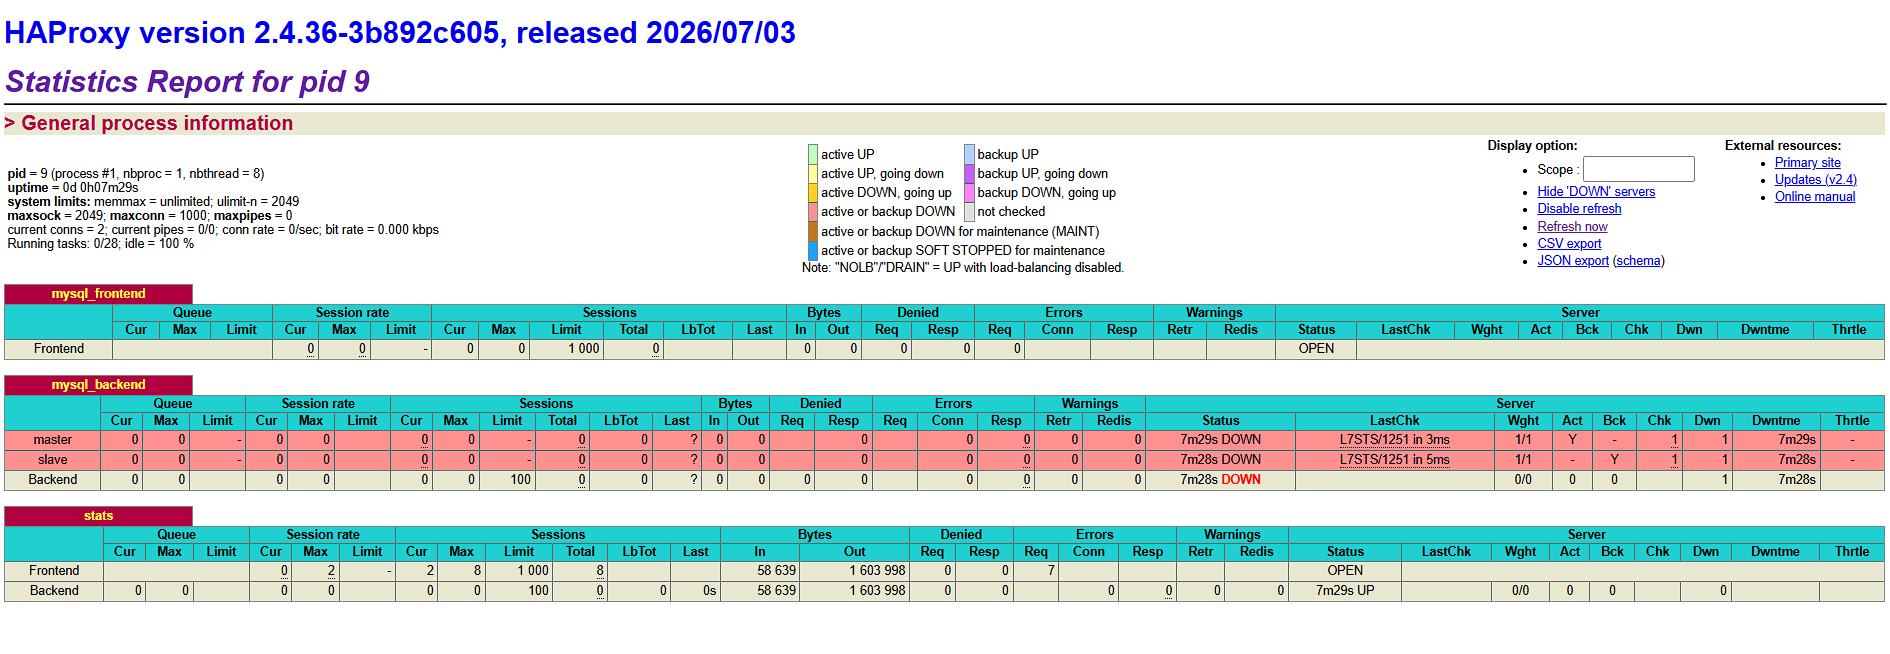
\includegraphics[width=0.85\textwidth]{../../../Archivos/Imagen/LocalHost_Docker.png}
    \caption{Localhost}
\end{figure}


\newpage
\subsection{Configuración de Permisos para HAProxy (Health Checks)}

Se creó un usuario dedicado sin contraseña y sin privilegios, cuyo único propósito es responder al ping del balanceador.

\vspace{2mm}

\textbf{1. Actualizar la configuración de HAProxy}
En el archivo \texttt{haproxy.cfg}, se sustituyó el usuario \texttt{root}:
\begin{lstlisting}
    option mysql-check user root
    
    option mysql-check user haproxy_check
\end{lstlisting}

\vspace{2mm}

\textbf{2. Crear el usuario en los motores MySQL}
Debido a incompatibilidades de encriptación entre HAProxy y MySQL 8.0, se forzó el método de autenticación \texttt{mysql\_native\_password} al crear el usuario en ambos contenedores.

\textit{Para el Maestro:}
\begin{lstlisting}[language=bash]
docker exec -it mysql-master mysql -uroot -p-e "CREATE USER 'haproxy_check'@'%' IDENTIFIED WITH mysql_native_password BY ''; FLUSH PRIVILEGES;"
\end{lstlisting}

\textit{Para la Réplica:}
\begin{lstlisting}[language=bash]
docker exec -it mysql-slave mysql -uroot -p -e "CREATE USER 'haproxy_check'@'%' IDENTIFIED WITH mysql_native_password BY ''; FLUSH PRIVILEGES;"
\end{lstlisting}

\textbf{3. Aplicar los cambios en el Balanceador}
Se reinició el servicio para que HAProxy adoptara el nuevo usuario:
\begin{lstlisting}[language=bash]
docker compose restart haproxy
\end{lstlisting}

Tras la ejecución, el panel de estadísticas en \texttt{http://localhost:8404/stats} confirmó que ambos nodos pasaron a estado activo (UP).

\begin{figure}[H]
    \centering
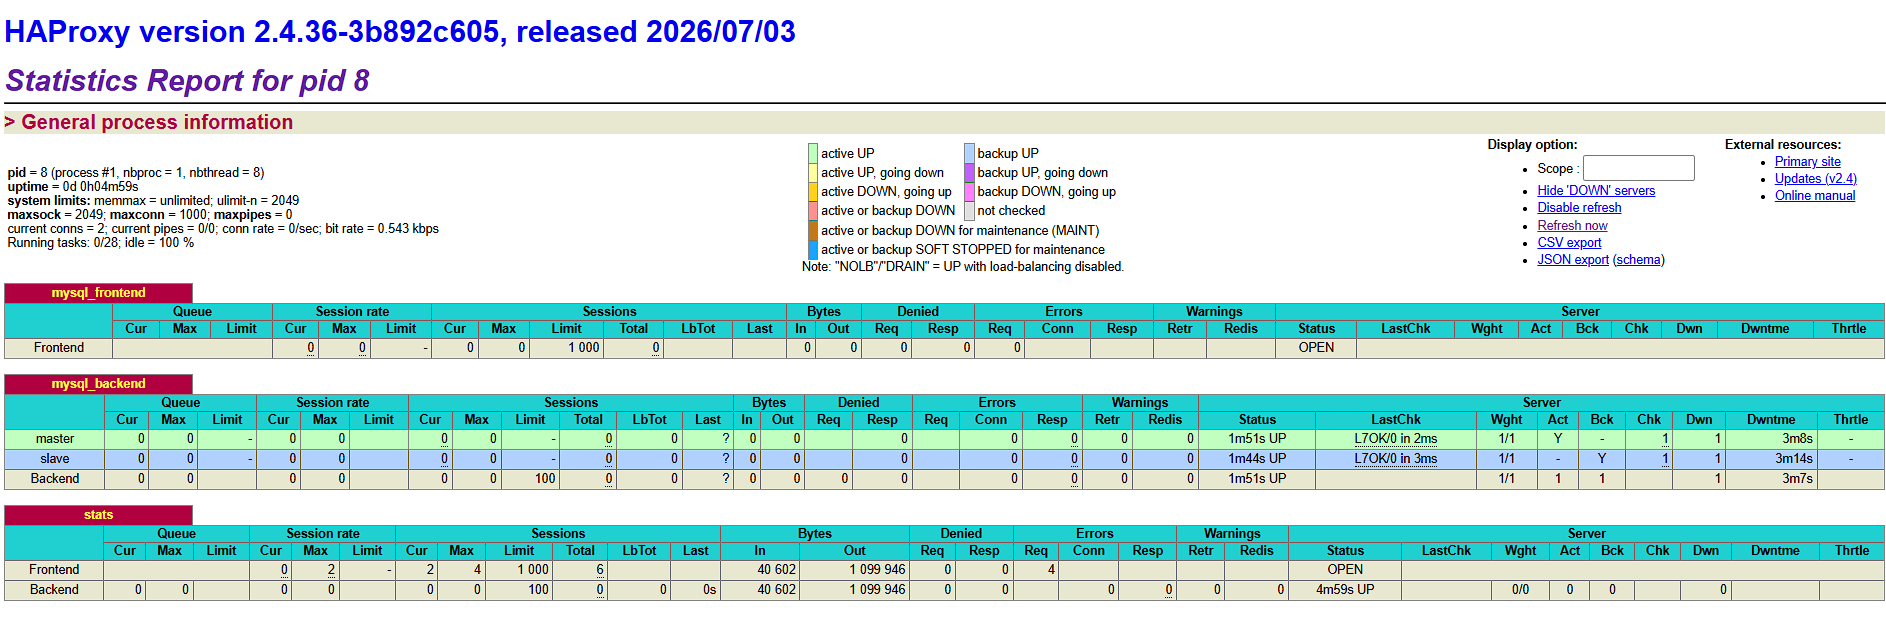
\includegraphics[width=0.85\textwidth]{../../../Archivos/Imagen/LocalHost_Docker_2.png}
    \caption{Localhost acceso a la base de datos (Estado UP)}
\end{figure}

\newpage
\subsection{Configuración de Replicación Maestro-Esclavo (GTID)}

Para el cumplimiento del diseño de Alta Disponibilidad, se implementó replicación asíncrona mediante GTID (Global Transaction Identifier). GTID es el estándar moderno en MySQL que facilita la sincronización, ya que cada transacción recibe un ID único y la réplica sabe exactamente qué eventos procesar sin requerir posiciones exactas de archivos \texttt{binlog}.

\subsubsection{Habilitar GTID y Replicación (Inyección vía Docker Compose)}

Debido a restricciones de seguridad en los permisos de volúmenes compartidos entre Windows y WSL (donde el motor ignora archivos de configuración con permisos demasiado abiertos), se optó por prescindir de los archivos físicos \texttt{mysqld.cnf}.

En su lugar, las variables de entorno para habilitar GTID se inyectaron directamente en la definición de cada contenedor dentro del archivo \texttt{docker-compose.yml} utilizando la directiva \texttt{command}.

\vspace{2mm}

\textbf{Configuración del Maestro en docker-compose.yml}
\begin{lstlisting}
    command: --server-id=1 --log-bin=mysql-bin --binlog-format=ROW --gtid-mode=ON --enforce-gtid-consistency=ON
\end{lstlisting}

\vspace{2mm}

\textbf{Configuración de la Réplica en docker-compose.yml}
\begin{lstlisting}
    command: --server-id=2 --gtid-mode=ON --enforce-gtid-consistency=ON --read-only=1
\end{lstlisting}

\subsubsection{Ejecución de la Arquitectura Limpia}
Para purgar configuraciones residuales y metadatos corruptos, se procedió a destruir el entorno anterior (incluyendo los volúmenes físicos de datos con el flag \texttt{-v}) y a instanciar la infraestructura en limpio:

\begin{lstlisting}[language=bash]
docker compose down -v
docker compose up -d
\end{lstlisting}

\subsubsection{Comandos de Replicación SQL}

\textbf{1. Obtener la IP interna del servidor Maestro}
La Réplica requiere enlazarse directamente a la dirección IP privada del contenedor Maestro dentro de la red virtual de Docker (\texttt{ecobici-net}).

\begin{lstlisting}[language=bash]
docker inspect -f '{{range.NetworkSettings.Networks}}{{.IPAddress}}{{end}}' mysql-master
\end{lstlisting}
\textit{Resultado:} \texttt{172.18.xxx}

\vspace{2mm}

\textbf{2. Crear el usuario de replicación en el Maestro}
\begin{lstlisting}[language=bash]
docker exec -it mysql-master mysql -uroot -p_xxxx
\end{lstlisting}

\begin{lstlisting}[language=SQL]
CREATE USER 'replica_user'@'%' IDENTIFIED WITH mysql_native_password BY 'xxx';
GRANT REPLICATION SLAVE ON *.* TO 'replica_user'@'%';
FLUSH PRIVILEGES;
EXIT;
\end{lstlisting}

\vspace{2mm}
\textbf{3. Conectar la Réplica al Maestro}
\begin{lstlisting}[language=bash]
docker exec -it mysql-slave mysql -uroot -p_xxx
\end{lstlisting}

\begin{lstlisting}[language=SQL]
CHANGE MASTER TO
  MASTER_HOST='xxx',
  MASTER_USER='replica_user',
  MASTER_PASSWORD='xxx',
  MASTER_AUTO_POSITION=1;
START SLAVE;
\end{lstlisting}

\subsubsection{Resolución de Incidentes: Error 1396 y Conflicto GTID}
Durante el proceso de conexión (\texttt{START SLAVE;}), el \textit{Coordinator worker} detuvo la clonación arrojando el error \texttt{Last\_SQL\_Errno: 1396} (\texttt{Operation CREATE USER failed}). Esto ocurrió porque el servidor esclavo intentó replicar una transacción DDL de creación de usuario que ya existía físicamente en su propio disco.

Para desatascar el flujo sin reconstruir el entorno, se aplicó una técnica avanzada de DBA inyectando un GTID vacío correspondiente a la transacción conflictiva, instruyendo al motor a omitirla y continuar con la cola de eventos.

\begin{lstlisting}[language=SQL]
STOP SLAVE;
SET GTID_NEXT="a8d9d588-cea3-11f1-ad19-0a3abf4f4181:7";
BEGIN;
COMMIT;
SET GTID_NEXT="AUTOMATIC";
START SLAVE;
\end{lstlisting}

Tras la corrección, la validación final mediante \texttt{SHOW SLAVE STATUS\textbackslash G} confirmó la sincronización exitosa de ambos hilos:
\begin{itemize}
    \item \texttt{Slave\_IO\_Running: Yes}
    \item \texttt{Slave\_SQL\_Running: Yes}
\end{itemize}

\newpage
\subsection{Cargar base de datos ECOBICI}

El contenedor mysql-master es un sistema operativo Linux aislado. No tiene disco C: ni identifica la ruta:
\begin{lstlisting}
    C:\ProgramData\MySQL\MySQL Server 8.0\Uploads.
\end{lstlisting}

para lo LOAD DATA INFILE del script.

\vspace{2mm}

Pasaremos los archivos de Windows al entorno de Linux en Docker y se modificaran las rutas.

\subsubsection{Copiar los archivos CSV al contenedor Linux}

\begin{lstlisting}
    docker cp "/mnt/c/ProgramData/MySQL/MySQL Server 8.0/Uploads/." mysql-master:/var/lib/mysql-files/
\end{lstlisting}

\subsubsection{Mover y modificar el script SQL}

Mover el archivo \texttt{QueryTS\_Ecobici\_CDMX.sql} a la carpeta del proyecto en Linux.

\begin{lstlisting}
\\wsl$\Ubuntu\home\ricardo\proyecto_ecobici.
\end{lstlisting}

\begin{lstlisting}
Buscar y Reemplazar
Buscar
C:/ProgramData/MySQL/MySQL Server 8.0/Uploads/
Reemplazar
/var/lib/mysql-files/
\end{lstlisting}

\subsubsection{Inyectar la base de datos}

En la terminal de Linux ejecuta el comando para inyectar todo el script directamente al maestro:

\begin{lstlisting}
    docker exec -i mysql-master mysql -uroot -p_xxxx DB_Ecobici_CDMX < QueryTS_Ecobici_CDMX.sql
\end{lstlisting}

\begin{alerta}{Importante}
Como este script carga más de 6 millones de registros y construye llaves foráneas e índices, el comando se quedará pensando durante unos 15 a 20 minutos. No lo canceles.
\end{alerta}

Si quieres ver cómo tu computadora está trabajando, puedes abrir una nueva pestaña o ventana de terminal en WSL y ejecutar el comando. Ahí verás en tiempo real cómo el contenedor mysql-master está utilizando al máximo tu CPU y memoria RAM.

\begin{lstlisting}
    docker stats.
\end{lstlisting}

\begin{figure}[H]
    \centering
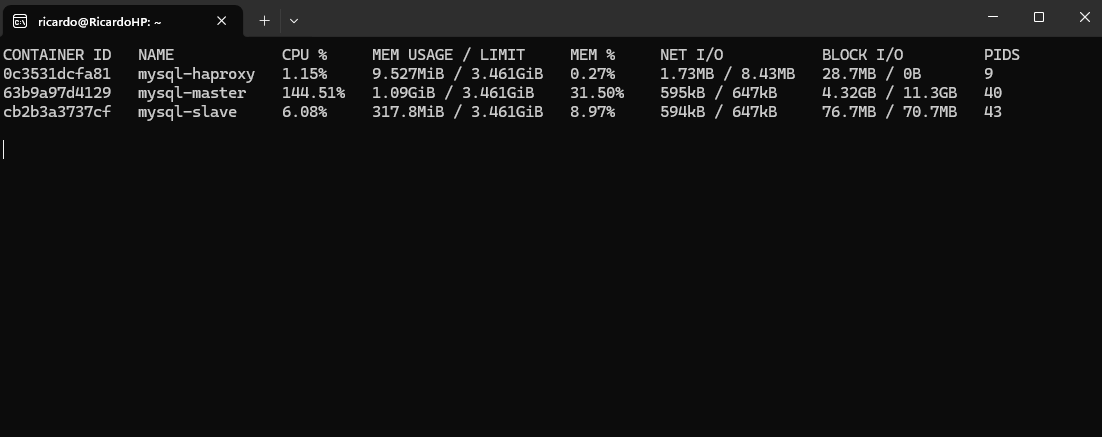
\includegraphics[width=0.85\textwidth]{../../../Archivos/Imagen/Docker_stats.png}
    \caption{Estatus carga}
\end{figure}

\newpage
\section{Crear Cuenta Google Cloud GCP.}

\begin{figure}[H]
    \centering
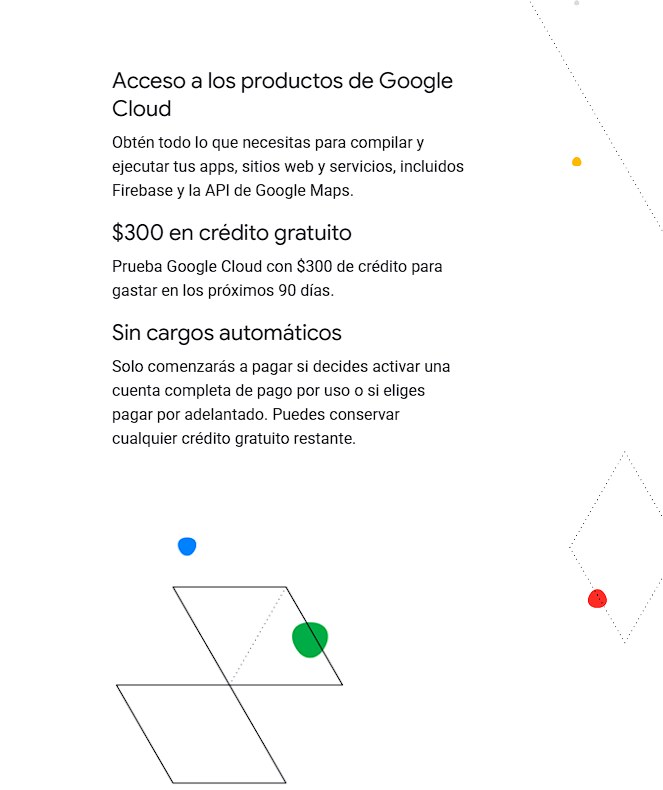
\includegraphics[width=0.85\textwidth]{../../../Archivos/Imagen/Acceso_GCP.png}
    \caption{GCP}
\end{figure}

\newpage

\subsection{Crear Instancias}

\begin{itemize}
    \item Ingresa a la Consola de Google Cloud.
    \item En el menú de navegación ve a Compute Engine > Instancias de VM.
    \item Haz clic en Crear instancia (Create instance).
    \item Configura los siguientes parámetros:
        Nombre: nodo-respaldo-ecobici
        Región: Selecciona us-central1 (Iowa)
        Tipo de máquina: Propósito general, serie E2, selecciona e2-micro (Es la opción más barata).
\end{itemize}


\begin{figure}[H]
    \centering
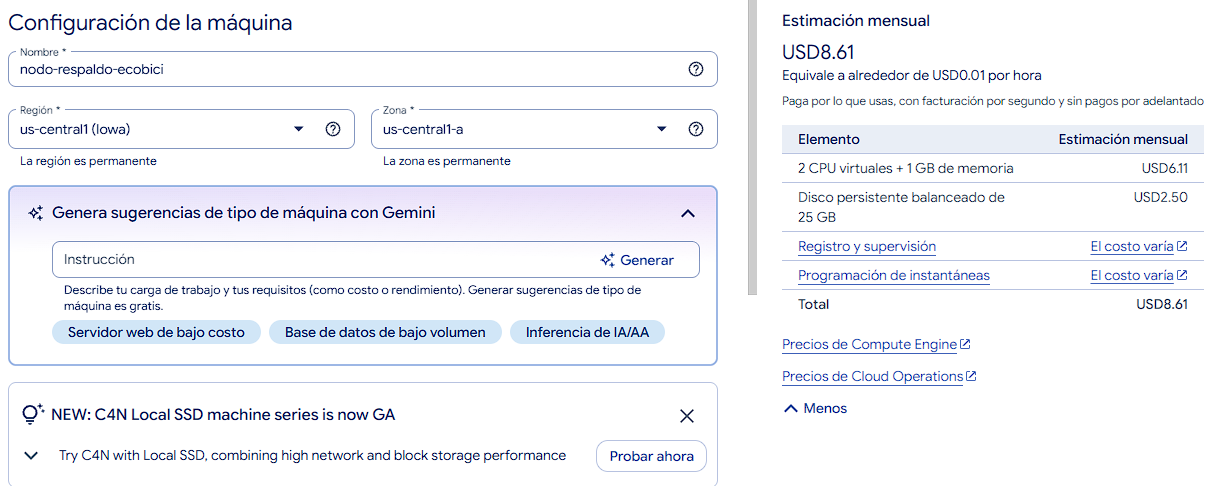
\includegraphics[width=0.85\textwidth]{../../../Archivos/Imagen/Configuracion_MV.png}
    \caption{Cofg mv}
\end{figure}


\begin{itemize}
    \item Disco de arranque (Boot disk):
    Haz clic en Cambiar.
    Sistema Operativo: Selecciona Ubuntu.
    Versión: Selecciona Ubuntu 24.04 LTS.
\end{itemize}


\begin{figure}[H]
    \centering
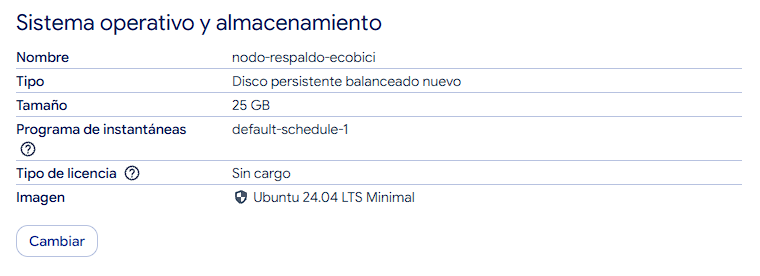
\includegraphics[width=0.85\textwidth]{../../../Archivos/Imagen/SO_MV.png}
    \caption{Cof SO}
\end{figure}

Tamaño: 10 GB (por defecto).
Firewall: Marca la casilla Permitir tráfico HTTP y Permitir tráfico HTTPS. 

\begin{figure}[H]
    \centering
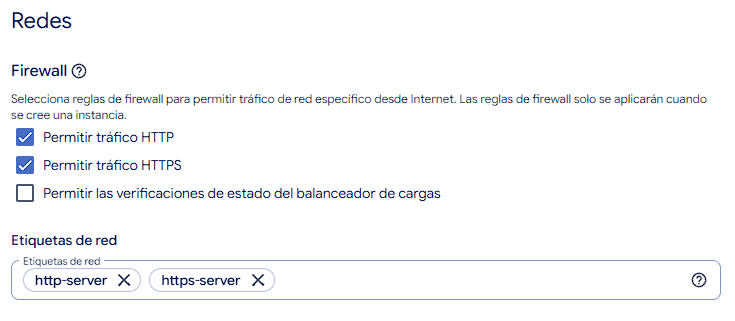
\includegraphics[width=0.85\textwidth]{../../../Archivos/Imagen/Firewall_MV.png}
    \caption{Firewall}
\end{figure}

Haz clic en el botón azul Crear al final de la página.

\newpage

\subsubsection{Regla de Firewall adicional}
Las casillas HTTP/HTTPS que se marcaron abren los puertos 80 y 443. 
Pero necesitamos abrir los puertos específicos de la bases de datos 
(3306 y 8404).

\begin{itemize}
    \item En el submenú que se despliega, haz clic en Firewall.
    \item En la parte superior central de la pantalla de Firewall, busca y haz clic en el botón que dice CREAR REGLA DE FIREWALL (Create Firewall Rule).
    \item Nombre: allow-haproxy
    \item Dirección del tráfico: Entrada
    \item Acción: Permitir
    \item Destinos: Todas las instancias de la red
    \item Rangos IPv4 de origen: 0.0.0.0/0
    \item Puertos TCP: 3306,8404
\end{itemize}


\begin{figure}[H]
    \centering
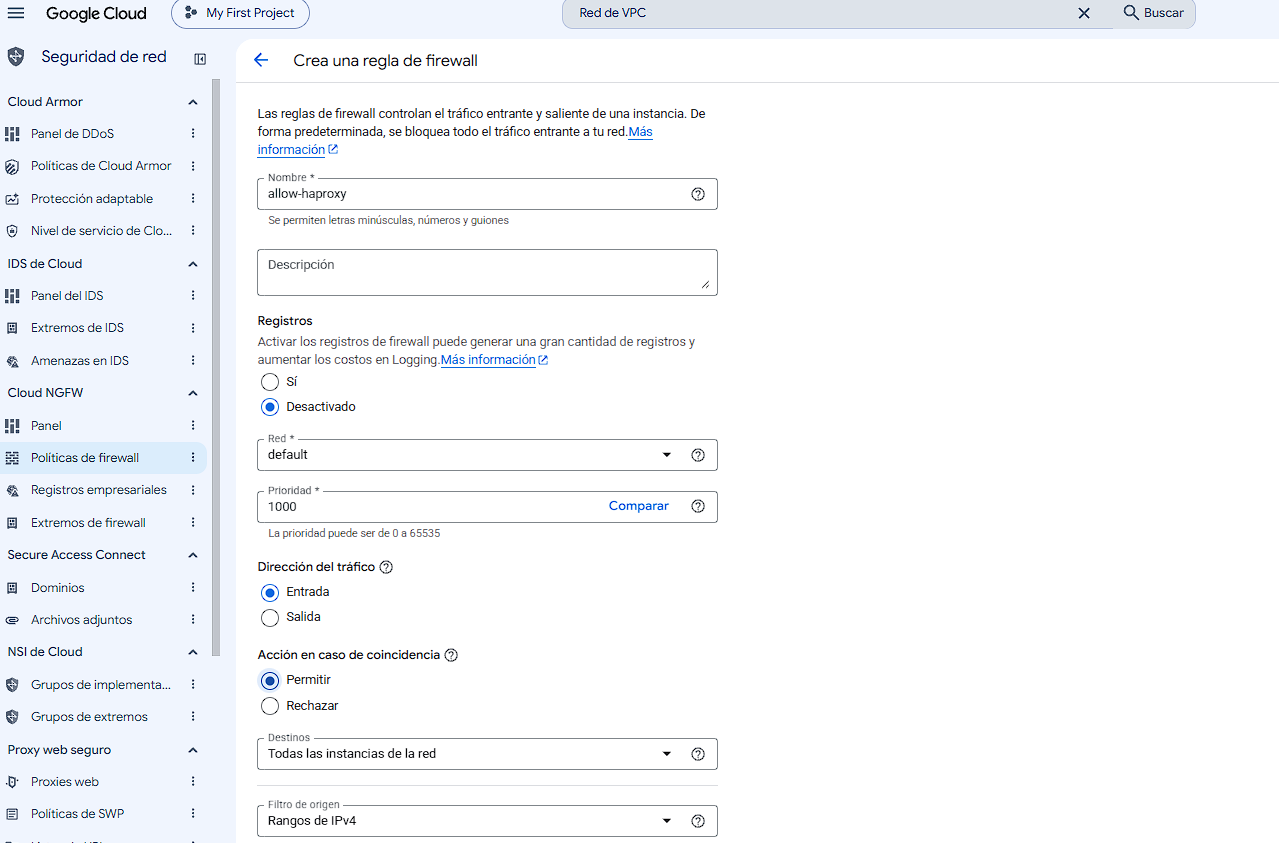
\includegraphics[width=0.85\textwidth]{../../../Archivos/Imagen/Firewall_Habilitar_1.png}
    \caption{Firewall}
\end{figure}

\begin{figure}[H]
    \centering
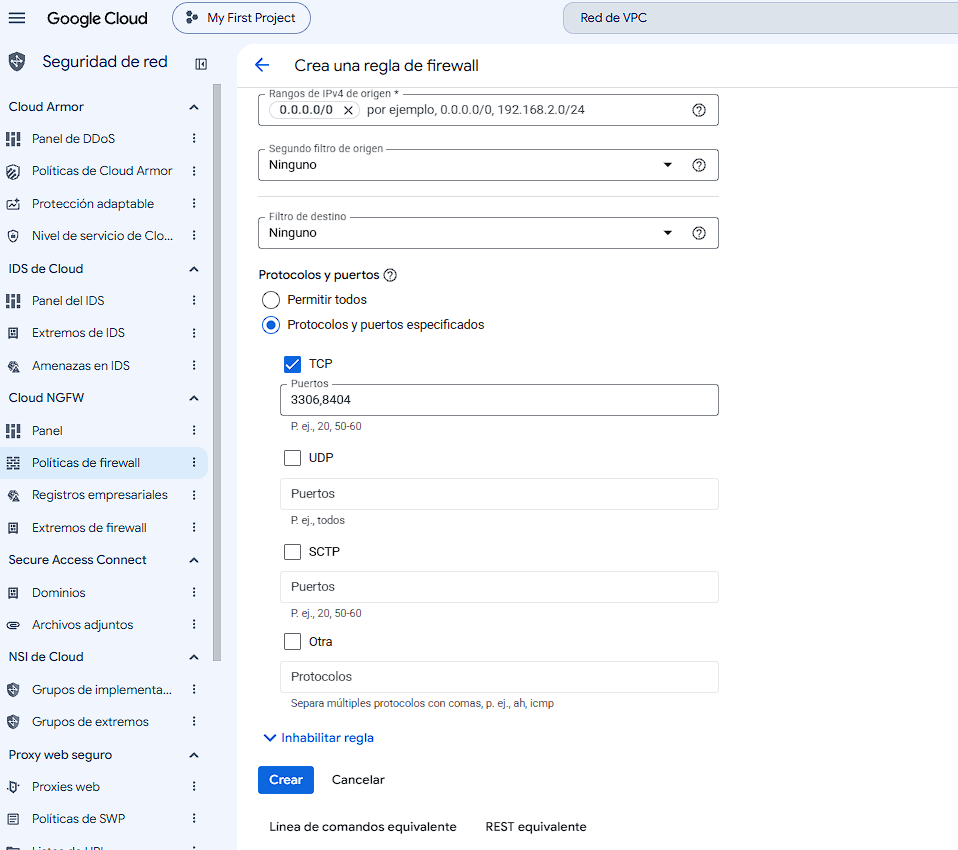
\includegraphics[width=0.85\textwidth]{../../../Archivos/Imagen/Firewall_Habilitar_2.png}
    \caption{Firewall}
\end{figure}

\vspace{2mm}

\newpage

\section{Maquina Virtual Cloud GCP.}

Maquina Virtual: Se observa la terminal de Ubuntu 2404 LTS conectada vá
SSH

\begin{figure}[H]
    \centering
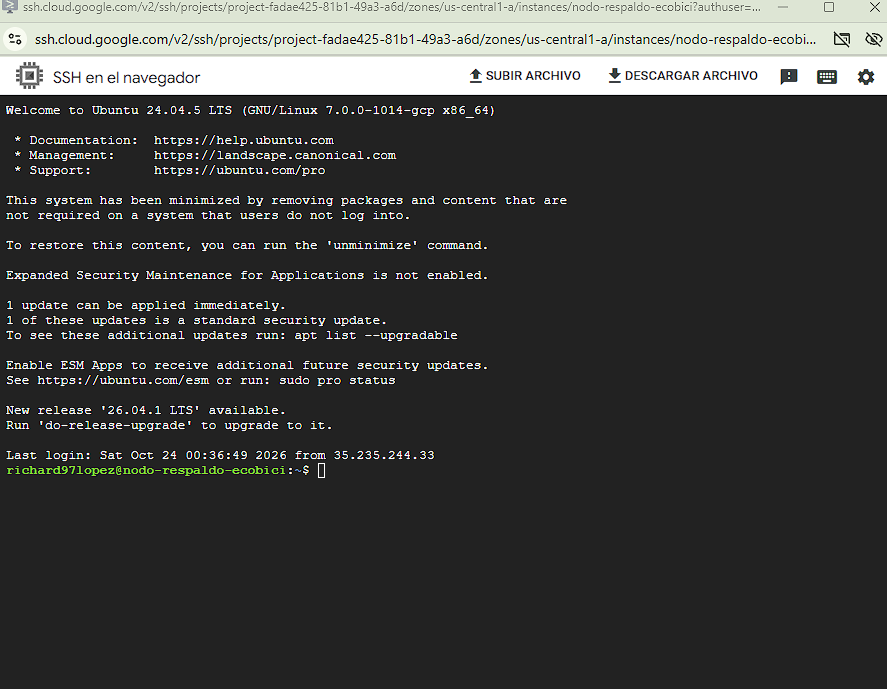
\includegraphics[width=0.85\textwidth]{../../../Archivos/Imagen/MV_SSH.png}
    \caption{Firewall}
\end{figure}

\section{Instalar Docker y Docker Compose Cloud GCP.}

Se instalara Docker en la maquina virtual y se caragra el proyecto

Primero actualizaremos los paquetes del sistema y luego instalaremos el motor de Docker.

\begin{lstlisting}
    sudo apt update && sudo apt upgrade -y
    sudo apt install docker.io docker-compose-v2 -y
\end{lstlisting}

\subsection{Dar permisos a tu usuario}

Para no tener que escribir sudo antes de cada comando de Docker, 
añadiremos tu usuario al grupo de Docker:

\begin{lstlisting}
    sudo usermod -aG docker $USER
    newgrp docker
\end{lstlisting}

\subsubsection{Crear la estructura del proyecto}

Crearemos las mismas carpetas que estan el localhost.

\begin{lstlisting}
    mkdir -p ~/proyecto_ecobici/haproxy
    cd ~/proyecto_ecobici
\end{lstlisting}

\subsubsection{Instalacion editor de texto nano}

\begin{lstlisting}
    sudo apt install nano -y
\end{lstlisting}

\vspace{2mm}

\subsubsection{Crear docker-compose.yml}
Arquitectura con GTID inyectado.
\begin{lstlisting}
    nano docker-compose.yml
\end{lstlisting}

\subsubsection{Crear haproxy.cfg}
La configuración del balanceador de carga dentro de su respectiva carpeta.
\begin{lstlisting}
    nano haproxy/haproxy.cfg
\end{lstlisting}

\section{Arrancar la infraestructura en la nube Cloud GCP.}
Con los archivos listos, ejecuta este comando para descargar las imágenes y encender los servidores de base de datos.
\begin{lstlisting}
    docker compose up -d
\end{lstlisting}

\vspace{2mm}

La arquitectura esta completa.
\begin{itemize}
    \item Maestro
    \item Esclavo
    \item HAProxy
\end{itemize}
Estan levantados los contenedores y de forma estable en la maquina 
virtual de GCP.

\subsection{Configuración de Permisos para HAProxy (Health Checks)}

La infraestructura funciona, los nodos de MySQL rechazan 
la conexión del balanceador porque todavía no se crea 
el usuario que HAProxy usa para verificar la salud de los 
servidores haproxy check.

Para el Maestro:
\begin{lstlisting}
    docker exec -it mysql-master mysql -uroot -p_ -e "DROP USER IF EXISTS 'haproxy_check'@'%'; CREATE USER 'haproxy_check'@'%' IDENTIFIED WITH mysql_native_password BY ''; FLUSH PRIVILEGES;"
\end{lstlisting}

Para la Réplica:
\begin{lstlisting}
   docker exec -it mysql-slave mysql -uroot -p_ -e "DROP USER IF EXISTS 'haproxy_check'@'%'; CREATE USER 'haproxy_check'@'%' IDENTIFIED WITH mysql_native_password BY ''; FLUSH PRIVILEGES;"
\end{lstlisting}

\begin{figure}[H]
    \centering
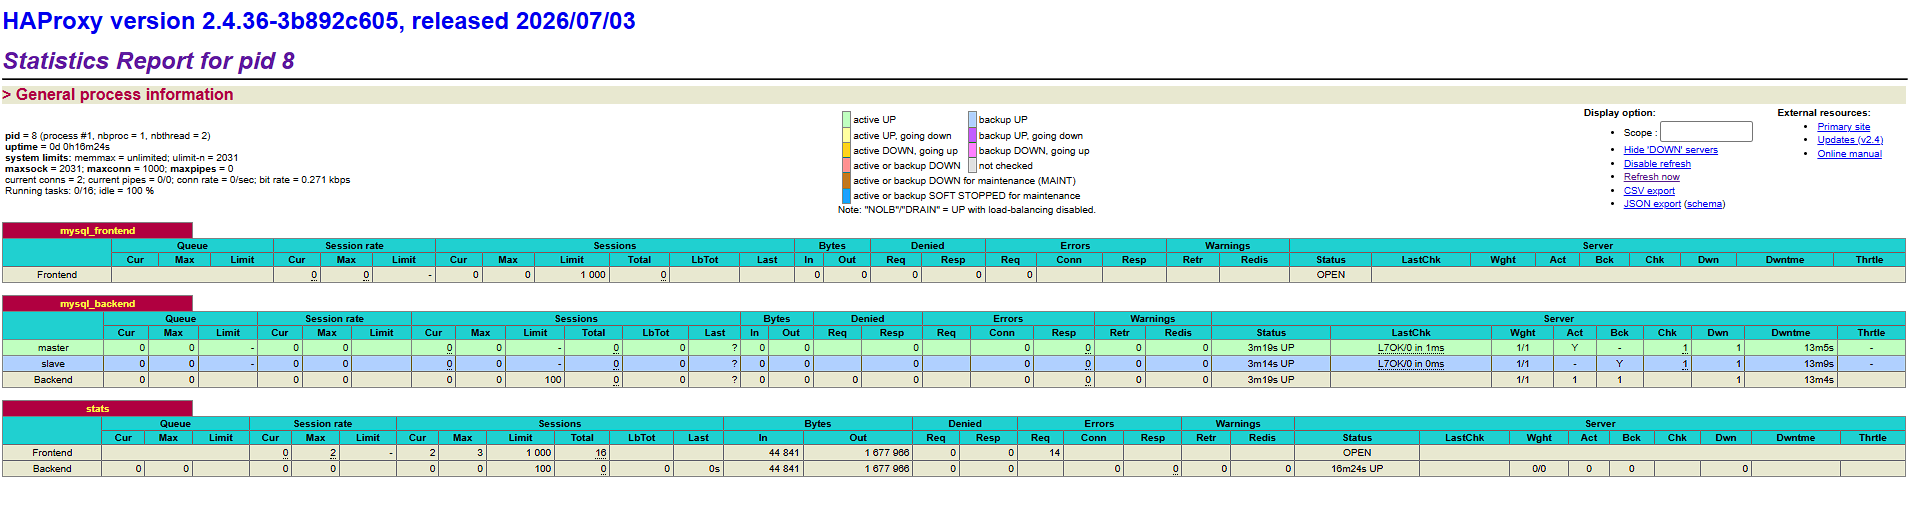
\includegraphics[width=0.85\textwidth]{../../../Archivos/Imagen/HAProxy_report_UP.png}
    \caption{HAProxy}
\end{figure}

\newpage

\subsubsection{Replicacion GTID}
IP interna del Maestro
\begin{lstlisting}
   docker inspect -f '{{range.NetworkSettings.Networks}}{{.IPAddress}}{{end}}' mysql-master
\end{lstlisting}

\subsubsection{Crear el usuario de clonación en el Maestro}
Entra a la terminal del Maestro:

\begin{lstlisting}
   docker exec -it mysql-master mysql -uroot -p_XXX
\end{lstlisting}
MySQL.
\begin{lstlisting}
    CREATE USER 'replica_user'@'%' IDENTIFIED WITH mysql_native_password BY 'xxx';
    GRANT REPLICATION SLAVE ON *.* TO 'replica_user'@'%';
    FLUSH PRIVILEGES;
    EXIT;
\end{lstlisting}


Conectar la Réplica al Maestro:

\begin{lstlisting}
   docker exec -it mysql-slave mysql -uroot -p_xxxx
\end{lstlisting}
MySQL.
\begin{lstlisting}
    STOP SLAVE;

    CHANGE MASTER TO
    MASTER_HOST='mysql-master',
    MASTER_USER='replica_user',
    MASTER_PASSWORD='xxxx',
    MASTER_AUTO_POSITION=1;

    START SLAVE;

    SHOW SLAVE STATUS\G
\end{lstlisting}

\subsubsection{Comprobar la conexión}

\begin{lstlisting}
   SHOW SLAVE STATUS\G
\end{lstlisting}

La replicación asíncrona por GTID está conectada y funcionando de 
forma estable. 

Se contruyo, desplego y estabilizo una arquitectura de Alta Disponibilidad
Master - Slave con balanceador de carga en HAProxy en GCP.

\newpage

\section{Poblar la Base de Datos Cloud GCP.}
Necesitas enviar el respaldo de tu esquema relacional local a la nube.
abriendo MySQL Workbench, localhost y creando una nueva conexión hacia tu instancia en GCP.

\begin{itemize}
    \item Host: 34.122.XXXX
    \item Puerto: XXXX.
    \item Contraseña: XXXX.
\end{itemize}

\begin{figure}[H]
    \centering
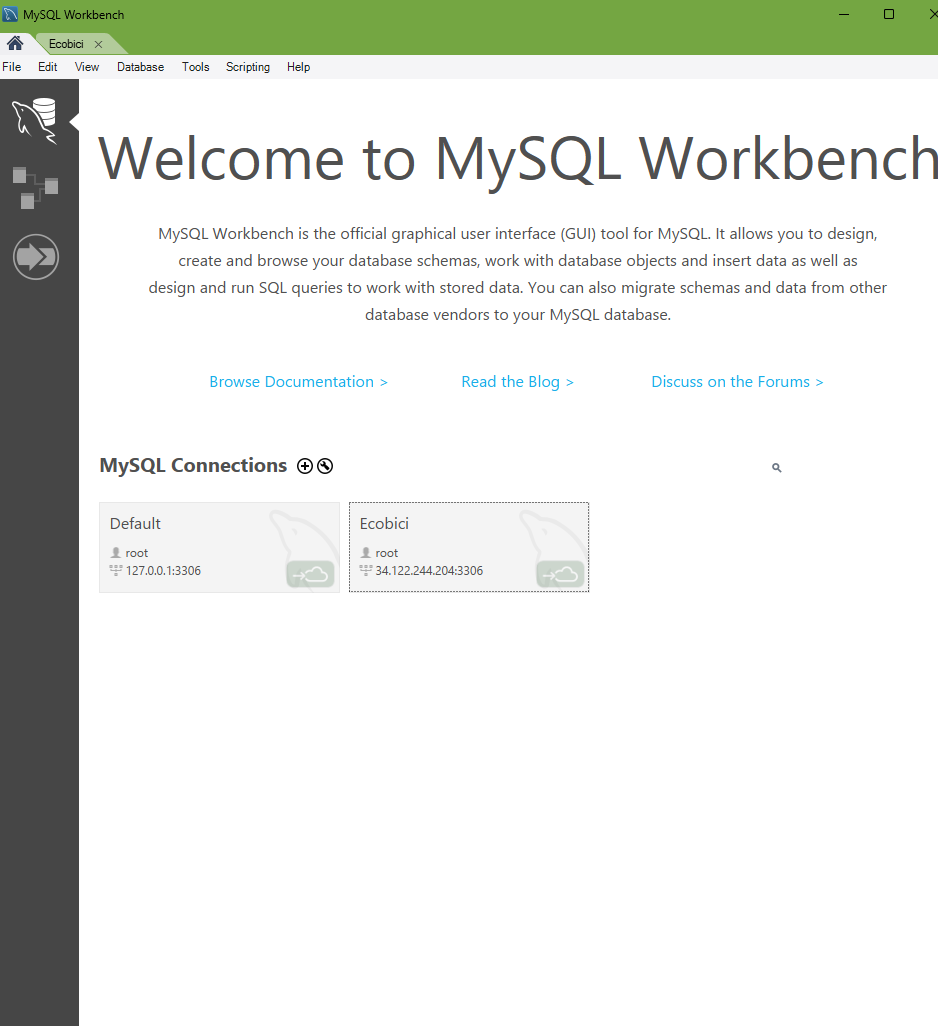
\includegraphics[width=0.85\textwidth]{../../../Archivos/Imagen/Conexion_workb.png}
    \caption{HAProxy}
\end{figure}

\newpage

\subsection{Cargar Data en la Maquina Virtual GCP}
Cargar la Data de Ecobici suben 12 archivos CSV a la nube.

\begin{figure}[H]
    \centering
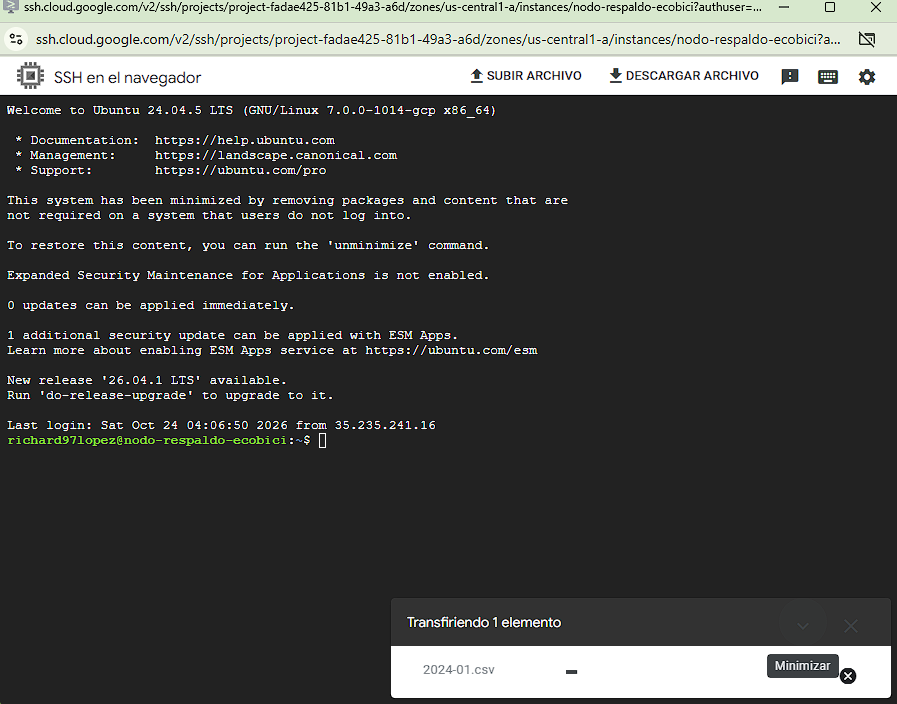
\includegraphics[width=0.85\textwidth]{../../../Archivos/Imagen/DATA_ecobici.png}
    \caption{Data}
\end{figure}

\subsubsection{Copiar dentro del contenedor Maestro}

Sedeben copiar dentro del contenedor Maestro usando el 
comando en tu terminal SSH:

\begin{lstlisting}
    docker cp *.csv mysql-master:/var/lib/mysql-files/
\end{lstlisting}

Finalmente, en MySQL Workbench, modifica todas las rutas de los archivos en tu script.
\begin{lstlisting}
     Cambia 
     C:/ProgramData/MySQL/
     por 
     /var/lib/mysql-files/nombre_del_archivo.csv.
\end{lstlisting}

Los 12 Archios CSV ya están alojados dentro del nodo Maestro en la ruta

\begin{figure}[H]
    \centering
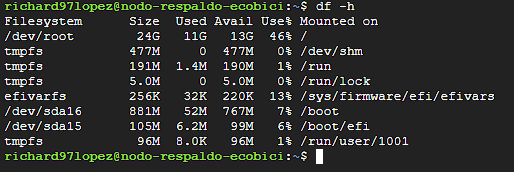
\includegraphics[width=0.85\textwidth]{../../../Archivos/Imagen/Inf_VM.png}
    \caption{VM}
\end{figure}

\newpage

\subsubsection{Ejecución del Script en MySQL Workbench}

\begin{itemize}
    \item Script QueryTS Ecobici CDMX en MySQL Workbench.
    \item Herramienta de Buscar y Reemplazar.
    \item Escribe la ruta exacta de Windows que tiene tu script actualmente.
    \begin{lstlisting}
        C:/ProgramData/MySQL/MySQL Server 8.0/Uploads/
    \end{lstlisting}
    \item Replace, escribe la nueva ruta de Linux.
    \begin{lstlisting}
        /var/lib/mysql-files/
    \end{lstlisting}
    \item Ejecutar todo el script
\end{itemize}

\begin{figure}[H]
    \centering
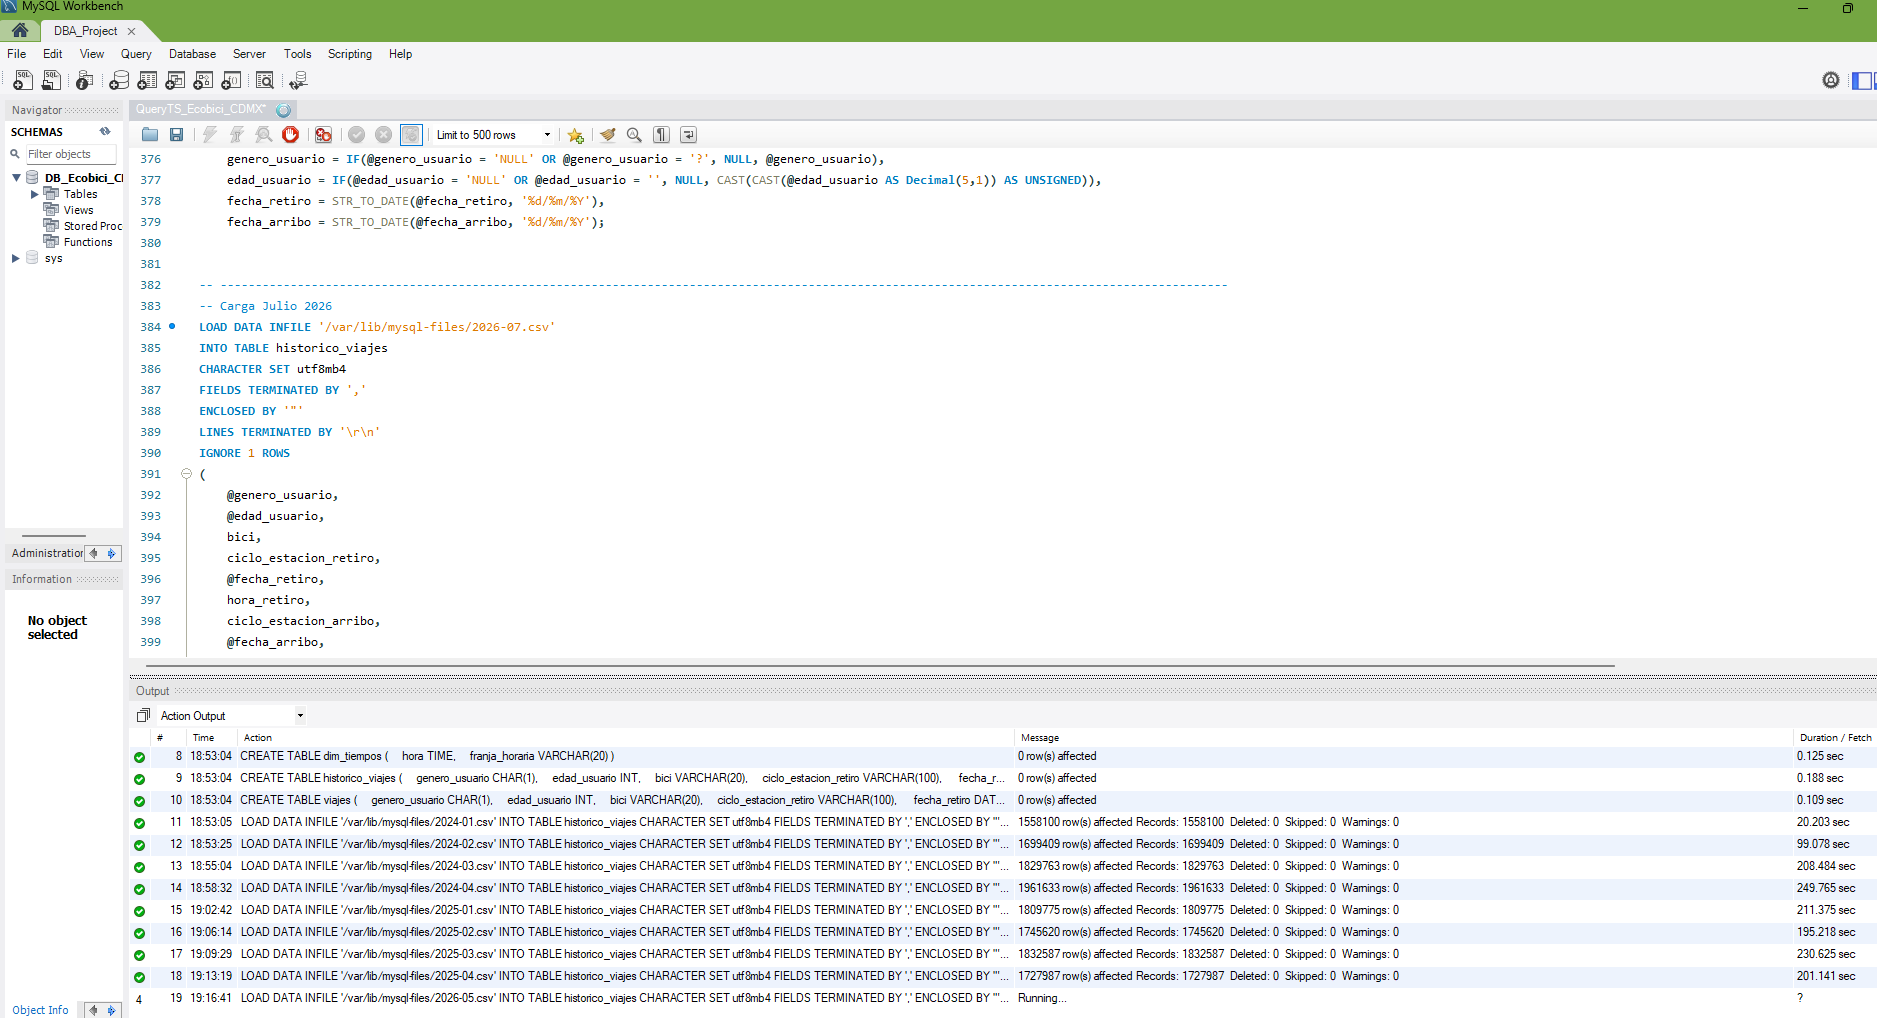
\includegraphics[width=0.85\textwidth]{../../../Archivos/Imagen/Ejecucion_script.png}
    \caption{VM}
\end{figure}

\subsubsection{PRIMARY KEY}

Se agregan las llaves primarias.

\begin{lstlisting}
    ALTER TABLE cat_generos ADD PRIMARY KEY (codigo_genero);
    ALTER TABLE estaciones ADD PRIMARY KEY (id_estacion);
    ALTER TABLE bicicletas ADD PRIMARY KEY (bici);
    ALTER TABLE dim_usuarios ADD PRIMARY KEY (id_perfil);
    ALTER TABLE dim_fechas ADD PRIMARY KEY (fecha);
    ALTER TABLE dim_tiempos ADD PRIMARY KEY (hora);
\end{lstlisting}

\subsubsection{FOREIGN KEY}
\begin{lstlisting}
    ALTER TABLE viajes
        ADD CONSTRAINT fk_viajes_genero FOREIGN KEY (genero_usuario) REFERENCES cat_generos(codigo_genero),
        ADD CONSTRAINT fk_viajes_bici FOREIGN KEY (bici) REFERENCES bicicletas(bici),
        ADD CONSTRAINT fk_viajes_estacion_retiro FOREIGN KEY (ciclo_estacion_retiro) REFERENCES estaciones(id_estacion),
        ADD CONSTRAINT fk_viajes_estacion_arribo FOREIGN KEY (ciclo_estacion_arribo) REFERENCES estaciones(id_estacion),
        ADD CONSTRAINT fk_viajes_fecha_retiro FOREIGN KEY (fecha_retiro) REFERENCES dim_fechas(fecha),
        ADD CONSTRAINT fk_viajes_hora_retiro FOREIGN KEY (hora_retiro) REFERENCES dim_tiempos(hora);
\end{lstlisting}

\section{Configuracion de Parametros Cloud GCP.}
Tu instancia nodo-respaldo-ecobici tiene 1 GB de RAM total. 
La regla del 60 - 80 asume que hay un único servidor de base de datos instalado en el sistema operativo. 
Dado que tu entorno de Alta Disponibilidad corre dos contenedores MySQL (Maestro y Esclavo) 
junto con HAProxy en la misma máquina virtual.

Se asignaran 300MB a cada nodo, lo que en conjunto representara el 60 de la RAM de la maquina virtual.

Se crean las carpetas.


\begin{lstlisting}
    mkdir -p ~/proyecto_ecobici/master/conf/mysql.conf.d/
    mkdir -p ~/proyecto_ecobici/slave/conf/mysql.conf.d/
\end{lstlisting}


\subsection{Configurar el nodo Maestro}


\begin{lstlisting}
    nano ~/proyecto_ecobici/master/conf/mysql.conf.d/mysqld.cnf

    innodb_buffer_pool_size = 300M
    innodb_log_buffer_size = 32M
\end{lstlisting}

\subsection{Configurar el nodo Esclavo}


\begin{lstlisting}
    nano ~/proyecto_ecobici/slave/conf/mysql.conf.d/mysqld.cnf

    innodb_buffer_pool_size = 300M
    innodb_log_buffer_size = 32M
    o
    echo -e "[mysqld]\ninnodb_buffer_pool_size = 300M\ninnodb_log_buffer_size = 32M" > ~/proyecto_ecobici/master/conf/mysql.conf.d/mysqld.cnf
\end{lstlisting}

\subsection{Aplicar los cambios en el clúster}

\begin{lstlisting}
    cd ~/proyecto_ecobici
    docker compose restart mysql-master mysql-slave

    o 
    echo -e "[mysqld]\ninnodb_buffer_pool_size = 300M\ninnodb_log_buffer_size = 32M" > ~/proyecto_ecobici/slave/conf/mysql.conf.d/mysqld.cnf
\end{lstlisting}

Verificar.

\begin{lstlisting}
    SHOW VARIABLES LIKE 'innodb_buffer_pool_size';
\end{lstlisting}

\begin{figure}[H]
    \centering
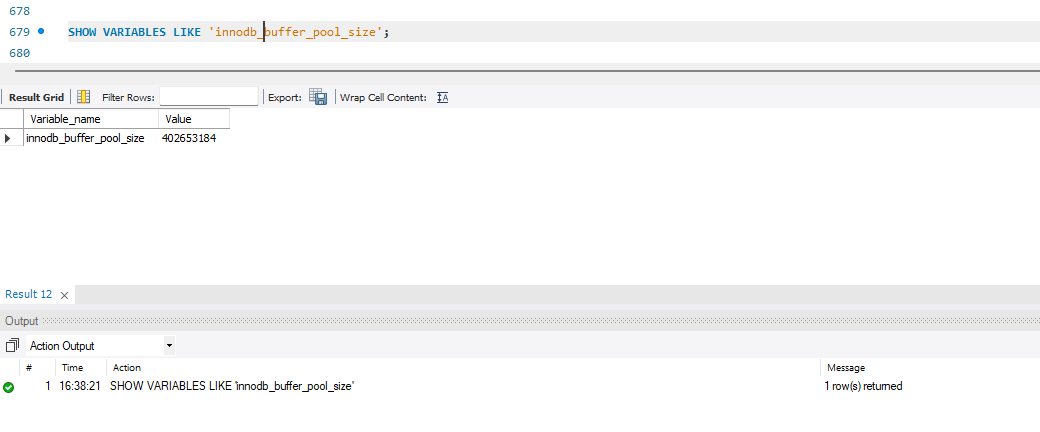
\includegraphics[width=0.85\textwidth]{../../../Archivos/Imagen/fuffer_pool.png}
    \caption{buffer pool}
\end{figure}

\newpage

\section{Disponibilidad y Automatizacion Cloud GCP.}

\subsection{Instalar la herramienta cron}

\begin{lstlisting}
sudo apt update && sudo apt install cron -y
\end{lstlisting}

\begin{lstlisting}
sudo systemctl enable --now cron
\end{lstlisting}

Crear un script de Bah en el servidor Ubuntu que ejecute
\begin{lstlisting}
    mysqldump 
con la bandera
    --single-transaction
\end{lstlisting}
Para no bloquear escrituras durante el respaldo y se automatizara con cron
para que se ejecute solo en la madrugada.

\subsection{Crear la carpeta y el script de respaldo}

\begin{lstlisting}
    mkdir ~/proyecto_ecobici/backups
    nano ~/proyecto_ecobici/backup.sh
\end{lstlisting}

\subsubsection{Script de automatización}

\textbf{--source-data=2}
\begin{lstlisting}
    !/bin/bash
    Script de Respaldo Logico para Ecobici CDMX

    FECHA=$(date +"%Y-%m-%d_%H-%M")
    DESTINO="/home/richard97lopez/proyecto_ecobici/backups/ecobici_full_$FECHA.sql"

    1. Ejecutar mysqldump a traves del contenedor Maestro
    docker exec mysql-master mysqldump -uroot -pxxx --single-transaction --source-data=2 --routines --events --triggers DB_Ecobici_CDMX > $DESTINO

    2. Comprimir el respaldo para no saturar el disco de 10 GB de GCP
    gzip $DESTINO
\end{lstlisting}

\subsubsection{Dar permisos y programar la tarea automática}
El script sea ejecutable.

\begin{lstlisting}
    chmod +x ~/proyecto_ecobici/backup.sh
\end{lstlisting}

\begin{lstlisting}
    crontab -e
\end{lstlisting}
Si te pregunta qué editor usar, presiona 1 para nano

Al final del archivo y  indica en la línea a 
Linux que ejecute tu script todos los días a las 2:00 AM hora del servidor.
\begin{lstlisting}
   0 2 * * * /home/richard97lopez/proyecto_ecobici/backup.sh
\end{lstlisting}

\subsubsection{Comprobar el peso del respaldo}
Para verificar físicamente que el script que acabas de 
ejecutar funcionó y comprimió tus 6.5 millones de viajes.

\begin{lstlisting}
    ls -lh ~/proyecto_ecobici/backups/
\end{lstlisting}

\subsection{Respaldo Incremental Diario (Binlogs)}

El script copiará la bitácora de transacciones (binlogs) todos los días,
permitiendo recuperar la base de datos hasta un segundo exacto 
antes de un accidente (Point-In-Time Recovery).

\begin{lstlisting}
    mkdir -p ~/proyecto_ecobici/backups/binlogs
    mkdir -p ~/proyecto_ecobici/logs
\end{lstlisting}

\begin{lstlisting}
    nano ~/proyecto_ecobici/respaldo_binlogs.sh
\end{lstlisting}

\begin{lstlisting}
    !/bin/bash
Respaldo incremental diario de binlogs
DIR=$HOME/proyecto_ecobici
DESTINO=$DIR/backups/binlogs
MYSQL="docker exec mysql-master mysql -uroot -p_xxx-N -e"

1. Rotacion: cerrar el binlog actual y abrir uno nuevo
$MYSQL "FLUSH BINARY LOGS;"

2. Identificar el binlog activo (no se copia)
ACTIVO=$($MYSQL "SHOW MASTER STATUS;" | awk '{print $1}')

3. Copiar los binlogs cerrados que aun no esten respaldados
for f in $(docker exec mysql-master bash -c "ls /var/lib/mysql | grep -E '^mysql-bin\.[0-9]+$'"); do
    if [ "$f" != "$ACTIVO" ] && [ ! -f "$DESTINO/$f" ]; then
        docker cp mysql-master:/var/lib/mysql/$f $DESTINO/
        echo "$(date) Binlog copiado: $f" >> $DIR/logs/respaldos.log
    fi
done

4. Conservar 14 dias de binlogs respaldados
find $DESTINO -name "mysql-bin.*" -mtime +14 -delete
\end{lstlisting}

\begin{lstlisting}
    chmod +x ~/proyecto_ecobici/respaldo_binlogs.sh
\end{lstlisting}

\newpage


\subsection{Mantenimiento Preventivo Automatizado ANALYZE y OPTIMIZE}

Para desfragmentar la base de datos limpiar los huecos que dejan los DELETE o UPDATE, 
se usara el programador interno de MySQL (Event Scheduler).

\subsubsection{MySQL Workbench}

Abre una nueva pestaña de consultas SQL y ejecuta el 
código exacto para crear el evento.

\begin{lstlisting}
    USE DB_Ecobici_CDMX;

    DELIMITER $$
    CREATE EVENT ev_mantenimiento_semanal
    ON SCHEDULE EVERY 1 WEEK
    STARTS CURRENT_TIMESTAMP
    COMMENT 'ANALYZE semanal y OPTIMIZE mensual (primer sabado)'
    DO
    BEGIN
        ANALYZE TABLE viajes, historico_viajes;
        IF DAYOFMONTH(CURRENT_DATE) <= 7 THEN
            OPTIMIZE TABLE viajes;
        END IF;
    END$$
    DELIMITER ;

    SELECT event_name, status, last_executed FROM information_schema.events WHERE event_schema = 'DB_Ecobici_CDMX';
\end{lstlisting}

\begin{figure}[H]
    \centering
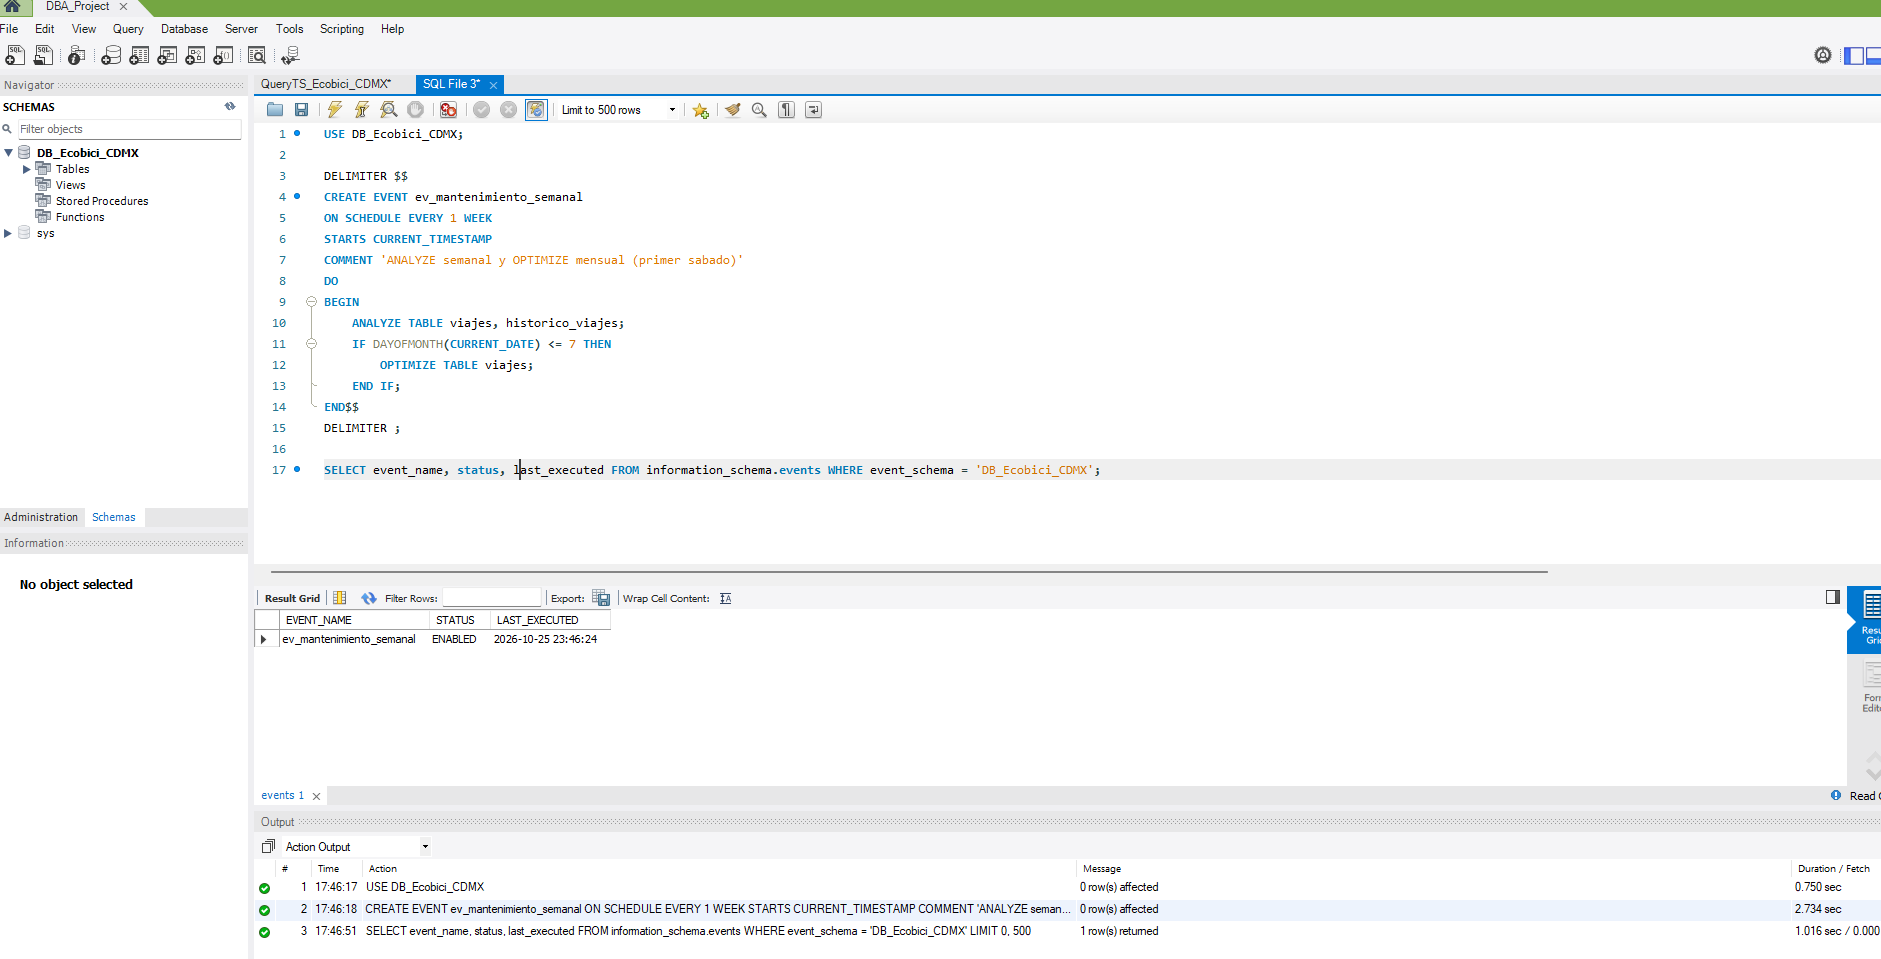
\includegraphics[width=0.85\textwidth]{../../../Archivos/Imagen/Event.png}
    \caption{CREATE EVENT}
\end{figure}

\newpage

\subsection{Rotación de Particiones y Retención de Datos}
La tabla histórica archive los datos viejos y que la tabla activa no crezca de forma descontrolada.

Se Crea el script de rotación en tu terminal

\begin{lstlisting}
    nano ~/proyecto_ecobici/rotacion_particiones.sh
\end{lstlisting}


\begin{lstlisting}
    !/bin/bash
    Rotacion mensual de particiones y generacion de resumen
    DIR=$HOME/proyecto_ecobici
    MYSQL="docker exec mysql-master mysql -uroot -p_xxx -DB_Ecobici_CDMX -N -e"

    Obtenemos el mes anterior (el que vamos a rotar)
    MES_A_ROTAR=$(date -d "last month" +"%Y%m")
    PARTICION="p_$MES_A_ROTAR"

    1. Resumir los datos antes de borrarlos
    $MYSQL "INSERT IGNORE INTO resumen_viajes_mes (anio, mes, ciclo_estacion_retiro, genero_usuario, total_viajes, edad_promedio, duracion_promedio_min)
    SELECT YEAR(fecha_retiro), MONTH(fecha_retiro), ciclo_estacion_retiro, IFNULL(genero_usuario, 'N'), COUNT(*), AVG(edad_usuario), AVG(TIME_TO_SEC(TIMEDIFF(hora_arribo, hora_retiro))/60)
    FROM historico_viajes PARTITION ($PARTICION)
    GROUP BY 1, 2, 3, 4;"

    2. Eliminar el detalle pesado
    $MYSQL "ALTER TABLE historico_viajes DROP PARTITION $PARTICION;"

    echo "$(date) Rotacion completada para $PARTICION" >> $DIR/logs/respaldos.log
\end{lstlisting}

\begin{lstlisting}
    chmod +x ~/proyecto_ecobici/rotacion_particiones.sh
\end{lstlisting}

\begin{figure}[H]
    \centering
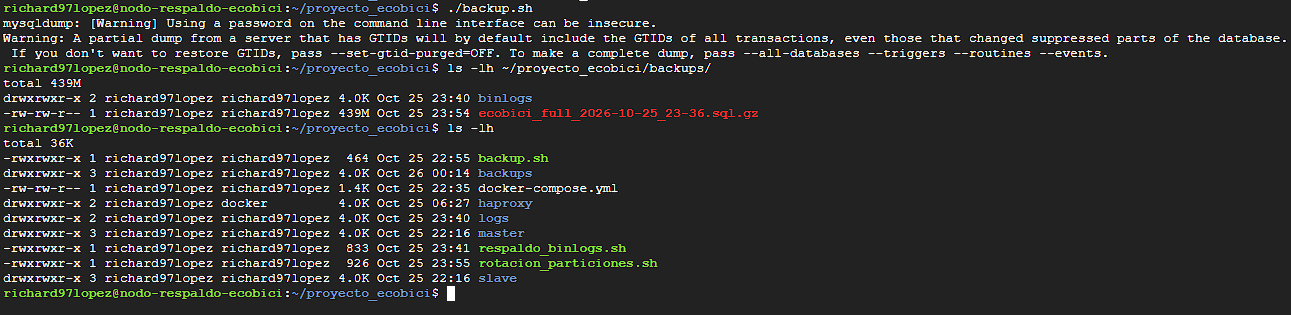
\includegraphics[width=0.85\textwidth]{../../../Archivos/Imagen/Backup.png}
    \caption{Pogramador de tareas}
\end{figure}


\newpage

\subsection{Programación de tareas(Cron) y Monitoreo}

\begin{figure}[H]
    \centering
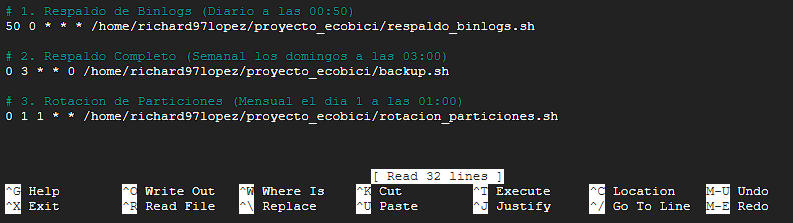
\includegraphics[width=0.85\textwidth]{../../../Archivos/Imagen/Programador_tareas.png}
    \caption{Pogramador de tareas}
\end{figure}


\end{document}